\documentclass[12pt,a4paper]{article}
\usepackage{amsmath}
\usepackage{amssymb} %mathbb
\usepackage{graphicx}
\usepackage{hyperref}
\usepackage{gensymb}
\usepackage{colortbl}
\usepackage{cancel}
\usepackage{amsthm}
\newtheorem{exercise}{Exercise}[section]
\newtheorem{defy}{Defiance}
\newtheorem{definition}{Definition}[section]
\newtheorem{thm}{Theorem}[section]
\newtheorem{example}{Example}[section]
\newtheorem*{solved}{Solved Exercise}
\newtheorem*{mainThm}{Main Theorem}
\newtheorem*{bonus}{Bonus}
\usepackage[top=1.0cm,bottom=1.3cm,left=1.0cm,right=1.0cm]{geometry}

\begin{document}

Main Video on \href{https://www.youtube.com/watch?v=V9X3EwOlvwg}{\color{blue}\underline{YouTube}}.

\Large

\vspace{6mm}

\textbf{Abstract}

\normalsize

\vspace{6mm}

Lambert functions, here, are almost equivalent to hypergeometric functions or theta functions | Glasser's derivations.

We know that an algebrical number is a kind of combination of radicals and such functions.

Our first intention is to pass through Galois's theorem and to solve $a_0 + a_1 x + \cdots + a_n x^n = 0$, for complex variable and for any natural $n$.

Our second intention to solve $a_0\cdot Id + a_1 T + \cdots + a_n T^n = 0$, for complex coefficients (or even in the commutator of $\mathcal{L}(\mathbb{R}^n)$) and square matrixes $T : \mathbb{R}^n \to \mathbb{R}^n$.

It is our third intention to translate smoothly one polynomial to another, by Girard's relations or Newton's identities.
(We have got uncountably many translations by Ordinary Differential Equations.)

It is our fourth intention to pass to exponentials and logarithms of matrixes.

It is our fifth intention to solve $e^z = z$.

It is our ambition to solve exactly $e^x = a_0 + a_1 x + a_2 x^2$, and also degrees greater than $2$.

It is our last intention to classify polynomials. By real or complex roots. And by multiplicity. Any degree. For each class, we intend to present an example.

\section{Bhaskara with Failure}

\begin{align}
&a,b,c,t\in \mathbb{R}\,;\,y:\mathbb{R}\to\mathbb{R}\,;\,r\in\mathbb{C} \\
a \cdot y''(t) + b\cdot y'(t) + c\cdot y(t) &= 0 \\
y &= c_1 ( \exp r_1 t) + c_2 ( \exp r_2 t ) \\
y' &= c_1 r_1 ( \exp r_1 t ) + c_2 r_2 (\exp r_2 t)  \\
y'' &= c_1 r_1^2 (\exp r_1 t) + c_2 r_2^2 (\exp r_2 t) \\
ar^2 + br + c &= 0 \\
ax^2 + bx + c &= 0 \\
 a\cdot y'' + b\cdot y' + c\cdot y &= 0 \\
 z_1 &= y \\
 z_2 &= y' \\
 Z' &= \left(\begin{matrix}0 & 1 \\ -c/a & -b/a \end{matrix}\right) \cdot Z \\
 Z &= \left[ \exp \left(\begin{matrix}0 & 1 \\ -c/a & -b/a \end{matrix}\right)t \right] \cdot C \\
 y &= C_1 \cdot f_1 + C_2 \cdot f_2 \\
 f_1 &\ne \exp r_1 t \\
 \ln f_1 &\ne r_1\cdot t \\
 r_1 &\ne \cfrac{1}{t}\cdot \ln f_1 \in \mathbb{C} \\
 r_2 &\ne \cfrac{1}{t}\cdot \ln f_2 \\
 \text{It would be better than  } r &= \cfrac{-b \pm \sqrt{b^2 - 4ac}}{2a} \\
 a x^2 + bx + c &= 0 \text{ would be solved.}
\end{align}

 \section{Quintic with Failure}

\begin{align}
\text{We would be ready to solve }ax^5 + b x^4 + c x^3 + d x^2 + e x + f &= 0 \\
a \cdot y^{(5)} + b \cdot y^{(4)}+ c \cdot y''' + d \cdot y'' + e \cdot y' + f &= 0 \\
 Z' = \left(\begin{matrix}0 & 1 & 0 & 0 & 0 \\ 0 & 0 & 1 & 0 & 0 \\ 0 & 0 & 0 & 1 & 0 \\ 0 & 0 & 0 & 0 & 1  \\ -f/a & -e/a & -d/a & -c/a & -b/a \end{matrix}\right) &\cdot Z \\
 Z &= [\exp tM] \cdot C \\
 y = C_1 \cdot f_1 + C_2 \cdot f_2 + C_3 \cdot f_3 + C_4 \cdot f_4 &+ C_5 \cdot f_5 \\
 f_i &\ne \exp r_i t \\
 r_i &\ne 1/t \cdot \ln f_i \in \mathbb{C}
\end{align}

\vspace{3mm}

For each polynomial $p(x)$, there are uncountably many equivalent equations of higher degree, multiples of $p(x)$. Better than no existing formula in radicals. Particularly, for all algebrical number, there is a series. The set of algebrical numbers is now a set of series.

But it's not only that. Roots have multiplicity.

\begin{align}
(x - r_1)^5 &= 0 \\
(x - r_1)^4 (x - r_2) &= 0 \\
(x - r_1)^3 (x - r_2)^2 &= 0 \\
(x - r_1)^3 (x - r_2)(x - r_3) &= 0 \\
(x - r_1)^2 (x - r_2)^2 (x - r_3) &= 0 \\
(x - r_1)^2 (x - r_2) (x - r_3)(x - r_4) &= 0 \\
\text{Suppose }r(t) &= t^{-1} \cdot \ln f \\
r'(t) &= - t^{-2} \cdot \ln f + t^{-1}\cdot 1/f \cdot f' = 0 \\
- f \ln f + t \cdot f' &= 0 \\
r\text{ would be a root if and only if Id } &= \cfrac{f \ln f}{f'}
\end{align}

\section{True Bhaskara with ODEs}

\begin{align}
Z &= \left[ \exp\, t M \right] \cdot C \\
Z &= \left[ \exp\, t \left(\begin{matrix}0 & 1 \\ -P & S \end{matrix}\right) \right] \cdot C \\
 y &= C_1 \cdot f_1 + C_2 \cdot f_2 \\
 y' &= C_1 \cdot f_1' + C_2 \cdot f_2' \\
 \left(\begin{matrix}f_1 & f_2 \\ f_1' & f_2' \end{matrix}\right) &= Id + tM + \cfrac{t^2}{2!}\cdot M^2 + \cfrac{t^3}{3!}\cdot M^3 + \cfrac{t^4}{4!}\cdot M^4 + \cdots \\
 \text{Let } &M_{ij}^n \text{ be the }(i,j)\text{-cell of the result of } M^n \nonumber \\
 f_1 &= 1 + t\underbrace{M_{11}}_{0} + \cfrac{t^2}{2!}\cdot M^2_{11} + \cfrac{t^3}{3!}\cdot M^3_{11} + \cfrac{t^4}{4!}\cdot M^4_{11} + \cdots \\
 f_1' &= 0 + tM_{21} + \cfrac{t^2}{2!}\cdot M^2_{21} + \cfrac{t^3}{3!}\cdot M^3_{21} + \cfrac{t^4}{4!}\cdot M^4_{21} + \cdots
\end{align}

\begin{align}
 f_2 &= 0 + t\underbrace{M_{12}}_{1} + \cfrac{t^2}{2!}\cdot M^2_{12} + \cfrac{t^3}{3!}\cdot M^3_{12} + \cfrac{t^4}{4!}\cdot M^4_{12} + \cdots \\
 f_2' &= 1 + tM_{22} + \cfrac{t^2}{2!}\cdot M^2_{22} + \cfrac{t^3}{3!}\cdot M^3_{22} + \cfrac{t^4}{4!}\cdot M^4_{22} + \cdots \\
 \exp xt &= 1 + t\cdot x + \cfrac{t^2}{2!}\cdot x^2 + \cfrac{t^3}{3!}\cdot x^3 + \cfrac{t^4}{4!}\cdot x^4 + \cdots \\
 \left(\begin{matrix}\exp{r_1 t} \\ \exp{r_2 t} \end{matrix}\right) &= \left(\begin{matrix}1 & r_1 \\ 1 & r_2 \end{matrix}\right) \cdot \left(\begin{matrix}f_1 \\ f_2 \end{matrix}\right) \\
E &= T F \\
 \left(\begin{matrix}\exp{r_1 t} & \exp{r_2 t} \\ r_1 \exp{r_1 t} & r_2 \exp{r_2 t} \end{matrix}\right) &= \exp tM \cdot T^\top \\
x^n &= M_{11}^n + x \cdot M_{12}^n \Leftarrow  x \in \{ r_1, r_2 \} = R \\
x^n &- x \cdot M_{12}^n - M_{11}^n = (x - r_1) \cdot (x - r_2) \cdot p_{n - 2}(x) \\
\exp xt &= f_1(t) + x\cdot f_2(t) \Leftarrow x \in R \\
x^3 &= (S^2 - P) x - PS \Leftarrow  x \in R\,;\,S = -b/a\,;\,P = c/a \\
x^4 &= (S^3 - 2 P S) x  + P(P - S^2) \Leftarrow  x \in R \\
x^5 &= (S^4 - 3 P S^2 + P^2) x + PS(2P - S^2) \Leftarrow  x \in R
\end{align}

\vspace{3mm}

Let's try to reduce \href{https://www.wolframalpha.com/input/?i=1+%3D+S*P*(2P+-+S%5E2);+1+%3D+S%5E4+-+3*+P*+S%5E2+%2B+P%5E2}{\color{blue}\underline{the equation}} $x^5 = x + 1$.

We've got two Bhaskaras, for each pair of complex solutions of the quintic.

\begin{align}
  \exp ntM &= \left(\begin{matrix}f_1(nt) & f_2(nt) \\ f_1'(nt) & f_2'(nt) \end{matrix}\right) = (\exp tM)^n
\end{align}

\begin{solved}
We see easily an expression for $\exp tM$ by means of $r_1, r_2$. With Bhaskara, write down an expression for $\exp tM$ by means of $S, P$. Sketch below:
\end{solved}

\begin{align}
T^{-1} &= \cfrac{1}{r_2 - r_1} \cdot \left(\begin{matrix}r_2 & -r_1 \\ -1 & 1 \end{matrix}\right) \\
\therefore \exp tM &=  \cfrac{1}{r_2 - r_1} \cdot \left(\begin{matrix}\exp{r_1 t} & \exp{r_2 t} \\ r_1 \exp{r_1 t} & r_2 \exp{r_2 t} \end{matrix}\right) \left(\begin{matrix}r_2 & -1 \\ -r_1 & 1 \end{matrix}\right)
\end{align}

\subsection{Companion Matrix $2$}

\begin{align}
  0 &= M^2 - S\cdot M + P\cdot\text{ Id } \\
  M^n &= \begin{pmatrix} M_{11}^n & M_{12}^n \\ M^{n+1}_{11} & M^{n+1}_{12} \end{pmatrix} \\
  \exp tM &= f_1(t) + f_2(t) \cdot M \\
  J(k) &= \left( \begin{matrix} 0 & 2k\pi \\ -2k\pi & 0 \end{matrix}\right) \label{jota} \\
  \exp M &= \text{ Id } \Leftrightarrow M \in L = \left\{ \sum_{k \in K \subset \mathbb{Z}} \sum_{p_{ij}(k)} P_{p_{ij}} J_k P^{-1} \,;\, J(k) \in \mathcal{J}\,;\,\det P \ne 0 \right\} \\
  \exp M &= T \Leftrightarrow M = \ln T + L \\
  T^M &\in \{ \exp [M (\ln T + L)], \exp [(\ln T + L) M] \} \\
  T^M &= F_1(t) + F_2(t) \cdot M \\
  T^M &= F_1(t) + M \cdot F_2(t)
\end{align}

\begin{thm}
Logarithmizable matrixes are similar to $\left( \begin{matrix} a > 0 & 0 \\ 0 & b > 0 \end{matrix}\right)$ or $\left( \begin{matrix} a & b \\ -b & a \end{matrix}\right) \ne 0$ or $\left( \begin{matrix} a & a \\ 0 & a > 0 \end{matrix}\right)$.
\end{thm}

\begin{bonus}
Every Jordan matrix has a similar companion matrix. Reciprocally $\cdots$
\end{bonus}

(The identity is a Jordan matrix, of course, because it has complex form $z = a + bi\,;\,a = 1\,;\,b = 0$.)

We discovered these particularities above, after Equation ({\color{blue}\underline{\ref{exp_M}}}).

\begin{align}
  T^2 - ST + P &= 0 \\
  \left(T - \cfrac{1}{2}\cdot S \right)\left(T - \cfrac{1}{2}\cdot S \right) &= \cfrac{1}{4}\cdot S^2 - P = VD^2 V^{-1} \\
  TS &= ST \\
  T &= \cfrac{1}{2}\cdot S + VDV^{-1} \\
  D &= \sqrt{\left(\begin{matrix}a^2 & 0 \\ 0 & b^2 \end{matrix}\right)} \,\vee\,\sqrt{\left(\begin{matrix}a^2 & 2a \\ 0 & a^2 \end{matrix}\right)} \,\vee\,\sqrt{\left(\begin{matrix}a^2 - b^2 & 2ab \\ -2ab & a^2 - b^2 \end{matrix}\right)}\,\vee\,\sqrt{a^2\cdot \text{Id}}
\end{align}

\subsection{From Exponential to Bhaskara}

\begin{align}
a + bx &= c^x \Leftarrow x \in \{ r_1, r_2 \} \Leftarrow x^2 - Sx + P = 0 \\
\exp t &= c \Rightarrow t = \ln c \\
f_1(\ln c) &= a = \cfrac{r_2 \cdot c^{r_1} - r_1 \cdot c^{r_2}}{r_2 - r_1} \\
f_2(\ln c) &= b = \cfrac{- c^{r_1} + c^{r_2}}{r_2 - r_1} \\
f_1'(\ln c) &= \cfrac{r_1 r_2 \cdot c^{r_1} - r_1 r_2 \cdot c^{r_2}}{r_2 - r_1} = - Pb \\
f_2'(\ln c) &= \cfrac{- r_1 \cdot c^{r_1} + r_2 \cdot c^{r_2}}{r_2 - r_1} = a + S b \\
\exp r_1 t + \exp r_2 t &= 2 f_1(t) + S f_2(t) \Rightarrow S = \cfrac{c^{r_1} + c^{r_2} - 2 a}{b} \\
x &= \cfrac{\exp xt - f_1(t)}{f_2(t)} \Rightarrow P = \cfrac{c^S - a (c^{r_1} + c^{r_2}) + a^2}{b^2} \\
P &= \cfrac{c^S - a^2 - abS}{b^2} \\
\Delta &= 0 \Leftrightarrow b^2 S^2 + 4 a^2 + 4 abS = 4 c^S = (2a + bS)^2 \\
\left(\begin{matrix}0 & 1 \\ -P & S \end{matrix}\right) &= \log_c \left(\begin{matrix}a & b \\ - P b & a + S b \end{matrix}\right) \label{exp_M}
\end{align}

\begin{exercise}
$a + bx = c^x$ with $\Delta = 0$. Tangent line.
\end{exercise}

\begin{definition}
Lambert W-function: $z\cdot e^z = a \Leftrightarrow z = W(a)$
\end{definition}

\href{https://www,dropbox,com/s/vxc39f4obrmw2ix/wlambert,pdf?dl=0}{\color{blue}\underline{Portuguese:}} study my other file which is not translated yet. The subject is: generalized Lambert $W$ functions.

\begin{example} If any function is continuous from a compact to itself, then Brouwer fixed-point theorem holds.
\begin{align}
e^z = z \Leftrightarrow z &= p_1 \pm i q_1 = 0.318131505\cdots \pm i \cdot 1.337235701\cdots \nonumber \\
\vee\,z &= p_2 \pm i q_2 = 2.06227773\cdots \pm i \cdot 7.588631178\cdots \nonumber \\
\vee\,z &= p_3 \pm i q_3 = 2.653191974\cdots \pm i \cdot 13.94920833\cdots
\end{align}
\end{example}

		\begin{center}
		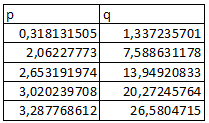
\includegraphics{tabelaPontoFixo}
		\end{center}

\begin{defy}
We still don't have a formula over $n$ for every $p + qi = - W_n(-1)$ above.
\end{defy}

There are countably many Bhaskaras for a single exponential.

For instance, $(x^2 - 4.124555460345492 x + 61.8403125981447) (x^2 - 0.63626301041114 x + 1.88940697578)$.

\begin{example} $\ln z = z$ | \href{https://github.com/boralaemcasa/propagation/blob/master/webs%20dot%20com/ufmg.htm}{\color{blue}\underline{claudino.webs.com/ufmg.htm}} | departamento anti Esp\'irito Santo
\end{example}

\begin{align}
\exp_k z &= z \\
e^z &= z \cdot e^{2k\pi i} \\
z &= \ln z \\
re^{it} &= \ln r + it + 2k\pi i \\
r \cos t &= \ln r \\
r \sin t &= t + 2k\pi \\
z &= - W(n, k, -1) \\
W : \mathbb{Z} \times \mathbb{Z} \times \mathbb{C} &\rightarrow \mathbb{C} \\
\overline{z} &= \ln \overline{z} \therefore W(1-n) = \overline{W(n)} \text{ defines } W(1,0,-1) \wedge W(2,0,-1) \\
W(-k) &= \overline{W(k)} \text{ defines }W\text{ for }k < 0
\end{align}

\begin{thm}
The real roots are the same.
\end{thm}

\begin{defy}
The (complex) solutions of the polynomial are extracted from the (complex) solutions of the exponential, modulo $m$. Define modulo $m$. (There is a problem only if $\Delta < 0$.)
\end{defy}

\begin{solved}
$z = 3^z/5 + 2/5 = f(z) \Leftrightarrow z_{1 - n} = - \cfrac{1}{\ln 3} \cdot W_n \left( - \cfrac{\ln 3}{5 \cdot \sqrt[5]{9}} \right) - \cfrac{2}{5}\,;\,n = 0 \vee n = -1$. \\
$\therefore z_1 = 1 < z_2 = 1.7124943083072217033\cdots \in \mathbb{R}$.
\end{solved}

\begin{exercise}
$w^z = z \Leftrightarrow z = \cfrac{\ln z}{\ln w} = (a + bi) \cdot \ln z \Leftrightarrow z_{1-n} = - \cfrac{W_n(- \ln w)}{\ln w}$.
\end{exercise}

\begin{thm}
$e^M = M \Leftrightarrow M = P\left(\begin{matrix}p & v \\ -q & u \end{matrix}\right) P^{-1}$, where $p + qi = \ln (p + qi) + A - Bi$, \\
$u + vi = \ln (u + vi) + D - Ci$, $\exp \left[ P^{-1}\left(\begin{matrix}A & B \\ C & D \end{matrix}\right) P \right] =$ Id.
\end{thm}

\begin{align}
e^{xu} &= ax + b \\
e^{xv} &= cx + d \\
c e^{xu} - a e^{xv} &= bc - ad \\
c \alpha^x - a \cdot \alpha^{2x} &= bc - ad \\
\alpha &= e^u \\
\beta &= e^v = \alpha^2 \\
y &= \alpha^x \\
a y^2 - c y + bc - ad &= 0 \\
y &= \cfrac{c \pm \sqrt{c^2 - 4a(bc - ad)}}{2a} \\
x &= \log_{\alpha} y
\end{align}

\begin{example}
$y^2 - 4 \cos(\ln 2)\cdot y + 4 = 0 \Leftrightarrow y = 2^{1 \pm i}$.
\end{example}

\begin{definition}
Bhaskara's family is $\mathcal{F}_2 \ni \{ x^n = ax + b\,;\,e^{xt} = ax + b\,;\,e^{2xt} - S(t) e^{xt} + P(t) = 0 \}$.
\end{definition}

\subsection{First-degree Lambert}

\begin{thm}
\begin{align}
e^{xt} &= ax + b\text{ with } \Delta > 0 \Leftrightarrow x_{1 - n} = \cfrac{1}{at} \left[ -aW_n \left( - \cfrac{t}{a \exp(bt/a)} \right) - bt \right]\,;\,n = 0 \vee n = -1
\end{align}
\end{thm}

\begin{mainThm}
Bhaskara $\Rightarrow$ Glasser. Therefore, every polynomial equation is solvable by generalized Glasser's derivations.
\end{mainThm}

\vspace{3mm}

Now, let's solve the quintic without radicals, and with whatever else, for instance, with Glasser.

 \section{True Quintic with ODEs}

\begin{align}
Z &= \left[ \exp\, t M \right] \cdot C \\
Z &= \left[ \exp\, t \left(\begin{matrix}0 & 1 & 0 & 0 & 0 \\ 0 & 0 & 1 & 0 & 0 \\ 0 & 0 & 0 & 1 & 0 \\ 0 & 0 & 0 & 0 & 1  \\ -f/a & -e/a & -d/a & -c/a & -b/a \end{matrix}\right) \right] \cdot C \\
 y &= C_1 \cdot f_1 + C_2 \cdot f_2 + C_3 \cdot f_3 + C_4 \cdot f_4 + C_5 \cdot f_5 \\
 y' &= C_1 \cdot f_1' + \cdots + C_5 \cdot f_5' \\
 y'' &= C_1 \cdot f_1'' + \cdots + C_5 \cdot f_5'' \\
 y''' &= C_1 \cdot f_1'''  + \cdots + C_5 \cdot f_5''' \\
 y'''' &= C_1 \cdot f_1''''  + \cdots + C_5 \cdot f_5'''' \\
 \left(\begin{matrix}f_1 & f_2 & f_3 & f_4 & f_5 \\ f_1' & f_2' & f_3' & f_4' & f_5' \\ f_1'' & f_2'' & f_3'' & f_4'' & f_5'' \\ f_1''' & f_2''' & f_3''' & f_4''' & f_5''' \\ f_1'''' & f_2'''' & f_3'''' & f_4'''' & f_5'''' \end{matrix}\right) &= Id + tM + \cfrac{t^2}{2!}\cdot M^2 + \cfrac{t^3}{3!}\cdot M^3 + \cfrac{t^4}{4!}\cdot M^4 + \cdots \\
 \text{Let } &M_{ij}^n \text{ be the }(i,j)\text{-cell of the result of } M^n \nonumber
\end{align}

\begin{align}
f_1 &= 1 + tM_{11} + \cfrac{t^2}{2!}\cdot M^2_{11} + \cfrac{t^3}{3!}\cdot M^3_{11} + \cfrac{t^4}{4!}\cdot \underbrace{M^4_{11}}_{0} + \cdots \\
f_2 &= 0 + tM_{12} + \cfrac{t^2}{2!}\cdot M^2_{12} + \cfrac{t^3}{3!}\cdot M^3_{12} + \cfrac{t^4}{4!}\cdot \underbrace{M^4_{12}}_{0} + \cdots \\
f_3 &= 0 + tM_{13} + \cfrac{t^2}{2!}\cdot M^2_{13} + \cfrac{t^3}{3!}\cdot M^3_{13} + \cfrac{t^4}{4!}\cdot \underbrace{M^4_{13}}_{0} + \cdots \\
f_4 &= 0 + tM_{14} + \cfrac{t^2}{2!}\cdot M^2_{14} + \cfrac{t^3}{3!}\cdot M^3_{14} + \cfrac{t^4}{4!}\cdot \underbrace{M^4_{14}}_{0} + \cdots \\
f_5 &= 0 + tM_{15} + \cfrac{t^2}{2!}\cdot M^2_{15} + \cfrac{t^3}{3!}\cdot M^3_{15} + \cfrac{t^4}{4!}\cdot \underbrace{M^4_{15}}_{1} + \cdots \\
&\text{Suppose that the multiplicity of every root is }1. \nonumber
\end{align}

\begin{align}
\exp xt &= 1 + t\cdot x + \cfrac{t^2}{2!}\cdot x^2 + \cfrac{t^3}{3!}\cdot x^3 + \cfrac{t^4}{4!}\cdot x^4 + \cdots \\
\left(\begin{matrix}\exp{r_1 t} \\ \exp{r_2 t} \\ \exp{r_3 t} \\ \exp{r_4 t} \\ \exp{r_5 t} \end{matrix}\right) &= \left(\begin{matrix}1 & r_1 & {r_1^2}/{2} & {r_1^3}/{6} & {r_1^4}/{24} \\ 1 & r_2 & {r_2^2}/{2} & {r_2^3}/{6} & {r_2^4}/{24} \\ 1 & r_3 & {r_3^2}/{2} & {r_3^3}/{6} & {r_3^4}/{24} \\ 1 & r_4 & {r_4^2}/{2} & {r_4^3}/{6} & {r_4^4}/{24} \\ 1 & r_5 & {r_5^2}/{2} & {r_5^3}/{6} & {r_5^4}/{24} \end{matrix}\right) \cdot \left(\begin{matrix}f_1 \\ f_2 \\ f_3 \\ f_4 \\ f_5 \end{matrix}\right) \\
E &= T F \\
\exp tM \cdot T^\top &= \left(\begin{matrix}\exp{r_1 t} & \exp{r_2 t} & \exp{r_3 t} & \exp{r_4 t} & \exp{r_5 t} \\ r_1 \exp{r_1 t} & r_2 \exp{r_2 t} & r_3 \exp{r_3 t} & r_4 \exp{r_4 t} & r_5 \exp{r_5 t}  \\ r_1^2 \exp{r_1 t} & r_2^2 \exp{r_2 t} & r_3^2 \exp{r_3 t} & r_4^2 \exp{r_4 t} & r_5^2 \exp{r_5 t} \\ r_1^3 \exp{r_1 t} & r_2^3 \exp{r_2 t} & r_3^3 \exp{r_3 t} & r_4^3 \exp{r_4 t} & r_5^3 \exp{r_5 t}  \\ r_1^4 \exp{r_1 t} & r_2^4 \exp{r_2 t} & r_3^4 \exp{r_3 t} & r_4^4 \exp{r_4 t} & r_5^4 \exp{r_5 t}  \end{matrix}\right)
 \end{align}

\begin{align}
x^n &= M_{11}^n + x \cdot M_{12}^n + \cfrac{x^2}{2} \cdot M_{13}^n + \cfrac{x^3}{6} \cdot M_{14}^n + \cfrac{x^4}{24} \cdot M_{15}^n \Leftarrow  x \in \{ r_1, r_2, r_3, r_4, r_5 \} = R \\
x^n &- \cfrac{x^4}{24} \cdot M_{15}^n - \cfrac{x^3}{6} \cdot M_{14}^n - \cfrac{x^2}{2} \cdot M_{13}^n - x \cdot M_{12}^n - M_{11}^n = \\
&= (x - r_1) \cdot (x - r_2) \cdot (x - r_3) \cdot (x - r_4) \cdot (x - r_5) \cdot p_{n - 5}(x) \\
\exp xt &= f_1(t) + x\cdot f_2(t) + \cfrac{x^2}{2} \cdot f_3(t) + \cfrac{x^3}{6} \cdot f_4(t) + \cfrac{x^4}{24} \cdot f_5(t) \Leftarrow x \in R
\end{align}

\vspace{3mm}

If there is a root with multiplicity $m > 1$, just derive it, solve the fourth degree one and find $\rho$. There is quintic$(\rho) = 0$. Divide the quintic by $x - \rho$ and solve the quartic.

\begin{exercise}
What are the \{transcendental numbers which are not representable by series\} ?
\end{exercise}

\begin{defy}
Multiplicity $m > 1$ and $z = a^z/k + bz^4/k + cz^3/k + dz^2/k + h/k = f(z)$.
After that, do the same thing with multiplicity $m = 1$.
\end{defy}

\begin{definition}
Quintic's family is $\mathcal{F}_5 \ni \{ x^n = ax^4 + bx^3 + cx^2 + dx + h\,;\,$ \\
$e^{xt} = ax^4 + bx^3 + cx^2 + dx + h\,;\,e^{5xt} - S_1(t) e^{4xt} + S_2(t) e^{3xt} - S_3(t) e^{2xt} + S_4(t) e^{xt} - P(t) = 0 \}$.
\end{definition}

\begin{align}
  \exp ntM &= \left(\begin{matrix}f_1(nt) & f_2(nt) & f_3(nt) & f_4(nt) & f_5(nt) \\ f_1'(nt) & f_2'(nt) & f_3'(nt) & f_4'(nt) & f_5'(nt) \\ f_1''(nt) & f_2''(nt) & f_3''(nt) & f_4''(nt) & f_5''(nt) \\ f_1'''(nt) & f_2'''(nt) & f_3'''(nt) & f_4'''(nt) & f_5'''(nt) \\ f_1''''(nt) & f_2''''(nt) & f_3''''(nt) & f_4''''(nt) & f_5''''(nt) \end{matrix}\right) = (\exp tM)^n
\end{align}

\begin{defy}
We see easily an expression for $\exp tM$ by means of $r_1, r_2, r_3, r_4, r_5$. Write down an expression for $\exp tM$ by means of $S_1, S_2, S_3, S_4, P$. (Do you see the impossibility by Galois's Theorem?) Sketch below:
\end{defy}

\begin{align}
\exp tM &=  \left(\begin{matrix}\exp{r_1 t} & \exp{r_2 t} & \exp{r_3 t} & \exp{r_4 t} & \exp{r_5 t} \\ r_1 \exp{r_1 t} & r_2 \exp{r_2 t} & r_3 \exp{r_3 t} & r_4 \exp{r_4 t} & r_5 \exp{r_5 t}  \\ r_1^2 \exp{r_1 t} & r_2^2 \exp{r_2 t} & r_3^2 \exp{r_3 t} & r_4^2 \exp{r_4 t} & r_5^2 \exp{r_5 t} \\ r_1^3 \exp{r_1 t} & r_2^3 \exp{r_2 t} & r_3^3 \exp{r_3 t} & r_4^3 \exp{r_4 t} & r_5^3 \exp{r_5 t}  \\ r_1^4 \exp{r_1 t} & r_2^4 \exp{r_2 t} & r_3^4 \exp{r_3 t} & r_4^4 \exp{r_4 t} & r_5^4 \exp{r_5 t}  \end{matrix}\right) \cdot \nonumber
\end{align}

\begin{align}
&\cdot \left(\begin{matrix}\cfrac{r_2 r_3 r_4 r_5}{\delta_{12}\delta_{13}\delta_{14}\delta_{15}} & -\cfrac{S_3(1)}{\delta_{12}\delta_{13}\delta_{14}\delta_{15}} & \cfrac{2S_2(1)}{\delta_{12}\delta_{13}\delta_{14}\delta_{15}}  & -6\cfrac{r_2 + r_3 + r_4 + r_5}{\delta_{12}\delta_{13}\delta_{14}\delta_{15}} & \cfrac{24}{\delta_{12}\delta_{13}\delta_{14}\delta_{15}}  \\ -\cfrac{r_1 r_3 r_4 r_5}{\delta_{12}\delta_{23}\delta_{24}\delta_{25}} & \cfrac{S_3(2)}{\delta_{12}\delta_{23}\delta_{24}\delta_{25}} & -\cfrac{2S_2(2)}{\delta_{12}\delta_{23}\delta_{24}\delta_{25}}  & 6\cfrac{r_1 + r_3 + r_4 + r_5}{\delta_{12}\delta_{23}\delta_{24}\delta_{25}} & -\cfrac{24}{\delta_{12}\delta_{23}\delta_{24}\delta_{25}} \\ \cfrac{r_1 r_2 r_4 r_5}{\delta_{13}\delta_{23}\delta_{34}\delta_{35}} & -\cfrac{S_3(3)}{\delta_{13}\delta_{23}\delta_{34}\delta_{35}} & \cfrac{2S_2(3)}{\delta_{13}\delta_{23}\delta_{34}\delta_{35}}  & -6\cfrac{r_1 + r_2 + r_4 + r_5}{\delta_{13}\delta_{23}\delta_{34}\delta_{35}} & \cfrac{24}{\delta_{13}\delta_{23}\delta_{34}\delta_{35}} \\ -\cfrac{r_1 r_2 r_3 r_5}{\delta_{14}\delta_{24}\delta_{34}\delta_{45}} & \cfrac{S_3(4)}{\delta_{14}\delta_{24}\delta_{34}\delta_{45}} & -\cfrac{2S_2(4)}{\delta_{14}\delta_{24}\delta_{34}\delta_{45}}  & 6\cfrac{r_1 + r_2 + r_3 + r_5}{\delta_{14}\delta_{24}\delta_{34}\delta_{45}} & - \cfrac{24}{\delta_{14}\delta_{24}\delta_{34}\delta_{45}} \\ \cfrac{r_1 r_2 r_3 r_4}{\delta_{15}\delta_{25}\delta_{35}\delta_{45}} & -\cfrac{S_3(5)}{\delta_{15}\delta_{25}\delta_{35}\delta_{45}} & \cfrac{2S_2(5)}{\delta_{15}\delta_{25}\delta_{35}\delta_{45}}  & -6\cfrac{r_1 + r_2 + r_3 + r_4}{\delta_{15}\delta_{25}\delta_{35}\delta_{45}} & \cfrac{24}{\delta_{15}\delta_{25}\delta_{35}\delta_{45}} \end{matrix}\right)
\end{align}

\subsection{Companion Matrix $5$}

\begin{align}
  0 &= M^5 - S\cdot M^4 + Q\cdot M^3 - T\cdot M^2 + U\cdot M - P\cdot\text{ Id } \\
   M^n &= \begin{pmatrix} M_{11}^n & M_{12}^n & M_{13}^n & M_{14}^n & M_{15}^n \\ M^{n+1}_{11} & M^{n+1}_{12} & M^{n+1}_{13}  & M^{n+1}_{14} & M^{n+1}_{15} \\ M^{n+2}_{11} & M^{n+2}_{12} & M^{n+2}_{13} & M^{n+2}_{14}& M^{n+1}_{15} \\ M^{n+3}_{11} & M^{n+3}_{12} & M^{n+3}_{13} & M^{n+3}_{14} & M^{n+3}_{15} \\ M^{n+4}_{11} & M^{n+4}_{12} & M^{n+4}_{13} & M^{n+4}_{14} & M^{n+4}_{15}  \end{pmatrix} \\
  \exp tM &= f_1(t) + f_2(t) \cdot M + \cfrac{f_3(t)}{2} \cdot M^2 + \cfrac{f_4(t)}{6} \cdot M^3 + \cfrac{f_5(t)}{24} \cdot M^4 \\
  \text{Definition } \ref{jota} \Rightarrow \Delta_{5 \times 5} &= \left\{ \left( \begin{matrix} 0 & 0 & 0 \\ 0 & J_1 & 0 \\ 0 & 0 & J_2 \end{matrix}\right), \left( \begin{matrix} J_1 & 0 & 0 \\ 0 & 0 & 0 \\ 0 & 0 & J_2 \end{matrix}\right), \left( \begin{matrix} J_1 & 0 & 0 \\ 0 & J_2 & 0 \\ 0 & 0 & 0 \end{matrix}\right)  \right\}
 \end{align}

\begin{align}
  \exp M &= \text{ Id } \Leftrightarrow M \in L = \left\{ \sum_{k_n \in K_n \subset \mathbb{Z}} \sum_{p_{ij}(k_n)} P_{p_{ij}} D_{k_n} P^{-1} \,;\, D(k_n) \in \Delta\,;\,\det P \ne 0 \right\} \\
  \exp M &= T \Leftrightarrow M = \ln T + L \\
  T^M &\in \{ \exp [M (\ln T + L)], \exp [(\ln T + L) M] \} \\
  T^M &= F_1(t) + F_2(t) \cdot M + \cfrac{F_3(t)}{2} \cdot M^2 + \cfrac{F_4(t)}{6} \cdot M^3 + \cfrac{F_5(t)}{24} \cdot M^4 \\
  T^M &= F_1(t) + M \cdot F_2(t) + M^2 \cdot \cfrac{F_3(t)}{2} + M^3 \cdot \cfrac{F_4(t)}{6} + M^4 \cdot \cfrac{F_5(t)}{24}
\end{align}

We have finished introduction. Next step is to work with degrees $1, 3, 4$ and, after that, turn back to degree $5$.

\section{From Exponential to Straight Line}

\begin{align}
x &= r_1 \Leftarrow \exp xt = \exp r_1 t = f_1(t) \\
a &= b^x \Leftarrow x \in \{ r_1 \} \Leftrightarrow x - S = 0 \\
S = r_1 &= \cfrac{\ln a + 2k\pi i}{\ln b}\,;\,k = 0 \\
\exp t &= b \Rightarrow t = \ln b \\
f_1(\ln b) &= a
\end{align}

\begin{definition}
Straight line's family is $\mathcal{F}_1 \ni \{ x^n = a\,;\,e^{xt} = a\,;\,e^{xt} - S(t) = 0 \}$.
\end{definition}

\subsection{Companion Matrix $1$}

\begin{align}
A(t) &= \exp t\cdot M \\
B(t) &= \exp t\cdot \text{ Id} \\
A(t) &= B(t)^M \\
\ln A(t) &\in \{ M \ln B(t), (\ln B(t))\cdot M \} \\
M &\in \{ (\ln A)(\ln B)^{-1}, (\ln B)^{-1}(\ln A) \} \text{ mod } L\,;\,\forall t \in \mathbb{R}\,;\,\exists\,!\,M \in \mathcal{L}(\mathbb{R}^n)
\end{align}

\section{From Exponential to Cubic}

\begin{align}
a + bx + cx^2 &= d^x \Leftarrow x \in \{ r_1, r_2, r_3 \} \Leftrightarrow x^3 - Sx^2 + Qx - P = 0 \\
\exp t &= d \Rightarrow t = \ln d \\
f_1(\ln d) &= a
\end{align}

\begin{align}
f_2(\ln d) &= b \\
f_3(\ln d)/2 &= c \\
\exp r_1 t + \exp r_2 t + \exp r_3 t &= 3 f_1(t) + S f_2(t) + (S^2/2 - Q) f_3(t) \\
S, Q, P &= \cdots \nonumber
\end{align}

\begin{defy}
$z = 4^z/5 - 3z^2/5 - 2/5 = f(z)$. \\
$z \in \mathbb{R} \Rightarrow z \in \{ -1.1433248602631500459\,;\,-0.35094297934554905880\,;\,2.5485570725290880406  \}$
\end{defy}

\begin{align}
e^{xu} &= a_0 + a_1 x + a_2 x^2 \\
e^{xv} &= b_0 + b_1 x + b_2 x^2 \\
b_2 \alpha^x - a_2 \beta^x &= b_2 (a_0 + a_1 x) - a_2 (b_0 + b_1 x) \\
\beta &= \alpha^2 \\
y &= \alpha^x \\
b_2 y - a_2 y^2 &= (b_2 a_1 - a_2 b_1)x + (b_2 a_0 - a_2 b_0) = L_1 x + L_0 \\
e^{xw} &= c_0 + c_1 x + c_2 x^2 \\
c_2 \alpha^x - a_2 \gamma^x &= c_2 (a_0 + a_1 x) - a_2 (c_0 + c_1 x) \\
\gamma &= \alpha^3 \\
c_2 y - a_2 y^3 &= (c_2 a_1 - a_2 c_1)x + (c_2 a_0 - a_2 c_0) = L_1' x + L_0' \\
- x &= (-b_2 y + a_2 y^2 + L_0)/L_1 = (-c_2 y + a_2 y^3 + L_0')/L_1' \\
0 &= (a_2/L_1') y^3 + (- a_2/L_1) y^2 + (b_2/L_1 - c_2/L_1') y + (L_0'/L_1' - L_0/L_1) \\
x &= \log_{\alpha} y
\end{align}

\begin{definition}
Cubic's family is $\mathcal{F}_3 \ni \{ x^n = ax^2 + bx + c\,;\,e^{xt} = ax^2 + bx + c\,;\,$ \\
$e^{3xt} - S_1(t) e^{2xt} + S_2(t) e^{xt} - P(t) = 0 \}$.
\end{definition}

\subsection{Second-degree Lambert}

\begin{align}
  e^{-cx} &= a(x^2 - Sx + P)\,;\,S = 0
\end{align}

\begin{align}
  x^2 - P &= w = W(z) \\
  x &= \pm \sqrt{w - P} \\
  e^{\mp c\sqrt{w - P}} &= aw \\
  \mp c\sqrt{w - P} &= \ln a + \ln w \\
  w e^w &= z \Rightarrow \ln w + w = \ln z \\
  c^2 (w - P) &= (\ln az - w)^2 \\
  0 &= w^2 - w(2 \ln az + c^2) + \ln^2 az + c^2 P \\
  w &= \cfrac{2 \ln az + c^2 \pm c \sqrt{c^2 + 4\ln az - 4 P}}{2}
\end{align}

\begin{align}
  \left( \cfrac{B + c \sqrt{\Delta}}{2} \right) e^{\cfrac{B}{2}} e^{\cfrac{c \sqrt{\Delta}}{2}} &= z = f(z) \\
  B &= 2 \ln az + c^2 \\
  \Delta &= c^2 + 4\ln az - 4 P
\end{align}

\section{From Exponential to Quartic}

\begin{align}
a + bx + cx^2 + dx^3 &= k^x \Leftarrow x \in \{ r_1, r_2, r_3, r_4 \} \Leftrightarrow x^4 - Sx^3 + Qx^2 - Tx + P = 0 \\
\exp t &= k \Rightarrow t = \ln k
\end{align}

\begin{align}
f_1(\ln k) &= a \\
f_2(\ln k) &= b \\
f_3(\ln k)/2 &= c \\
f_4(\ln k)/6 &= d \\
e^{r_1 t} + e^{r_2 t} + e^{r_3 t}  + e^{r_4 t} &= 4 f_1(t) + S f_2(t) + (S^2/2 - Q) f_3(t) + (S^3/6 - SQ/2 + T/2) f_4(t) \\
S, Q, T, P &= \cdots \nonumber
\end{align}

\begin{defy}
$(z + 2)(z + 3)(z + 4) = 5^z$. \\
$z \in \mathbb{R} \Rightarrow z \in \{ -3.9992\,;\,-3.0079\,;\,-1.97995\,;\,3.4634972226061445400 \}$
\end{defy}

\begin{align}
e^{xu} &= a_0 + a_1 x + a_2 x^2 + a_3 x^3 \\
e^{xv} &= b_0 + b_1 x + b_2 x^2 + b_3 x^3 \\
b_3 \alpha^x - a_3 \beta^x &= b_3 (a_0 + a_1 x + a_2 x^2) - a_3 (b_0 + b_1 x + b_2 x^2) \\
\beta &= \alpha^2 \\
y &= \alpha^x \\
b_3 y - a_3 y^2 &= (b_3 a_2 - a_3 b_2) x^2 + (b_3 a_1 - a_3 b_1)x + (b_3 a_0 - a_3 b_0) = L_2 x^2 + L_1 x + L_0 \\
e^{xw} &= c_0 + c_1 x + c_2 x^2 + c_3 x^3 \\
c_3 \alpha^x - a_3 \gamma^x &= c_3 (a_0 + a_1 x + a_2 x^2) - a_3 (c_0 + c_1 x + c_2 x^2) \\
\gamma &= \alpha^3
\end{align}

\begin{align}
c_3 y - a_3 y^3 &= (c_3 a_2 - a_3 c_2) x^2 + (c_3 a_1 - a_3 c_1)x + (c_3 a_0 - a_3 c_0) = L_2' x^2 + L_1' x + L_0' \\
x^2 &= (b_3 y - a_3 y^2 - L_1 x - L_0)/L_2 = (c_3 y - a_3 y^3 - L_1' x - L_0')/L_2' \\
x &= A_3 y^3 + A_2 y^2 + A_1 y + A_0 \\
e^{xt} &= d_0 + d_1 x + d_2 x^2 + d_3 x^3 \\
d_3 \alpha^x - a_3 \delta^x &= d_3 (a_0 + a_1 x + a_2 x^2) - a_3 (d_0 + d_1 x + d_2 x^2) \\
\delta &= \alpha^4 \\
d_3 y - a_3 y^4 &= (d_3 a_2 - a_3 d_2) x^2 + (d_3 a_1 - a_3 d_1)x + (d_3 a_0 - a_3 d_0) = L_2'' x^2 + L_1'' x + L_0'' \\
x^2 &= (b_3 y - a_3 y^2 - L_1 x - L_0)/L_2 = (d_3 y - a_3 y^4 - L_1'' x - L_0'')/L_2'' \\
x &= A_4' y^4 + A_2' y^2 + A_1' y + A_0' \\
0 &= y^4 + B_3 y^3 + B_2 y^2 + B_1 y + B_0 \\
x &= \log_{\alpha} y
\end{align}

\begin{definition}
Quartic's family is $\mathcal{F}_4 \ni \{ x^n = ax^3 + bx^2 + cx + d\,;\,e^{xt} = ax^3 + bx^2 + cx + d\,;\,$ \\
$e^{4xt} - S_1(t) e^{3xt} + S_2(t) e^{2xt} - S_3(t) e^{xt} + P(t) = 0 \}$.
\end{definition}

\section{From Exponential to Quintic}

\begin{align}
e^{xu} &= a_0 + a_1 x + a_2 x^2 + a_3 x^3 + a_4 x^4 \\
e^{xv} &= b_0 + b_1 x + b_2 x^2 + b_3 x^3 + b_4 x^4 \\
b_4 \alpha^x - a_4 \beta^x &= b_4 (a_0 + a_1 x + a_2 x^2 + a_3 x^3) - a_4 (b_0 + b_1 x + b_2 x^2 + b_3 x^3) \\
\beta &= \alpha^2 \\
y &= \alpha^x \\
b_4 y - a_4 y^2 &= (b_4 a_3 - a_4 b_3) x^3 + (b_4 a_2 - a_4 b_2) x^2 + (b_4 a_1 - a_4 b_1)x + (b_4 a_0 - a_4 b_0) = \nonumber \\
&= L_3 x^3 + L_2 x^2 + L_1 x + L_0 \\
e^{xw} &= c_0 + c_1 x + c_2 x^2 + c_3 x^3 + c_4 x^4 \\
c_4 \alpha^x - a_4 \gamma^x &= c_4 (a_0 + a_1 x + a_2 x^2 + a_3 x^3) - a_4 (c_0 + c_1 x + c_2 x^2 + c_3 x^3) \\
\gamma &= \alpha^3 \\
c_4 y - a_4 y^3 &= (c_4 a_3 - a_4 c_3)x^3 + (c_4 a_2 - a_4 c_2) x^2 + (c_4 a_1 - a_4 c_1)x + (c_4 a_0 - a_4 c_0) = \nonumber \\
&= L_3' x^3 + L_2' x^2 + L_1' x + L_0' \\
x^3 &= (b_4 y - a_4 y^2 - L_2 x^2 - L_1 x - L_0)/L_3 = (c_4 y - a_4 y^3 - L_2' x^2 - L_1' x - L_0')/L_3' \\
x^2 + A_4 x &= A_3 y^3 + A_2 y^2 + A_1 y + A_0 \\
e^{xt} &= d_0 + d_1 x + d_2 x^2 + d_3 x^3 + d_4 x^4 \\
d_4 \alpha^x - a_4 \delta^x &= d_4 (a_0 + a_1 x + a_2 x^2 + a_3 x^3) - a_4 (d_0 + d_1 x + d_2 x^2 + d_3 x^3) \\
\delta &= \alpha^4 \\
d_4 y - a_4 y^4 &= (d_4 a_3 - a_4 d_3) x^3 + (d_4 a_2 - a_4 d_2) x^2 + (d_4 a_1 - a_4 d_1)x + (d_4 a_0 - a_4 d_0) = \nonumber \\
&= L_3'' x^3 + L_2'' x^2 + L_1'' x + L_0'' \\
x^3 &= (b_4 y - a_4 y^2 - L_2 x^2 - L_1 x - L_0)/L_3 = (d_4 y - a_4 y^4 - L_2'' x^2 - L_1'' x - L_0'')/L_3'' \\
x^2 + A_5' x &= A_4' y^4 + A_2' y^2 + A_1' y + A_0' \\
x^2 &= A_3 y^3 + A_2 y^2 + A_1 y + A_0 - A_4 x = A_4' y^4 + A_2' y^2 + A_1' y + A_0' - A_5' x \\
x &= B_4 y^4 + B_3 y^3 + B_2 y^2 + B_1 y + B_0 \\
e^{xs} &= g_0 + g_1 x + g_2 x^2 + g_3 x^3 + g_4 x^4 \\
g_4 \alpha^x - a_4 \epsilon^x &= g_4 (a_0 + a_1 x + a_2 x^2 + a_3 x^3) - a_4 (g_0 + g_1 x + g_2 x^2 + g_3 x^3) \\
\epsilon &= \alpha^5
\end{align}

\begin{align}
g_4 y - a_4 y^5 &= (g_4 a_3 - a_4 g_3) x^3 + (g_4 a_2 - a_4 g_2) x^2 + (g_4 a_1 - a_4 g_1)x + (g_4 a_0 - a_4 g_0) = \nonumber \\
&= L_3''' x^3 + L_2''' x^2 + L_1''' x + L_0''' \\
x^3 &= (b_4 y - a_4 y^2 - L_2 x^2 - L_1 x - L_0)/L_3 = (g_4 y - a_4 y^5 - L_2''' x^2 - L_1''' x - L_0''')/L_3''' \\
x^2 + A_6'' x &= A_5'' y^5 + A_2'' y^2 + A_1'' y + A_0'' \\
x^2 &= A_3 y^3 + A_2 y^2 + A_1 y + A_0 - A_4 x = A_5'' y^5 + A_2'' y^2 + A_1'' y + A_0'' - A_6'' x \\
x &= B_5' y^5 + B_3' y^3 + B_2' y^2 + B_1' y + B_0' \\
0 &= y^5 + C_4 y^4 + C_3 y^3 + C_2 y^2 + C_1 y + C_0 \\
x &= \log_{\alpha} y
\end{align}

Next section, we fastly see why the quintic is unsolvable by radicals.

\section{Hungerford's Algebra}

\begin{definition}
Let $E$ and $F$ be extension fields of a field $K$. A nonzero map $\sigma: E \to F$ which is both a field and a $K$-module homomorphism is called a $K$-homomorphism.
\end{definition}

\begin{definition}
If a field automorphism $\sigma \in$ Aut $F$ is a $K$-homomorphism, then $\sigma$ is called a $K$-automorphism of $F$.
\end{definition}

\begin{definition}
The group of $\{\sigma\,;\, \sigma$ is $K$-automorphism of $F\}$ is called the Galois group of $F$ over $K$ and is denoted $\text{Aut}_K\,F$.
\end{definition}

\begin{definition}
Let $F$ be a field and $f \in F[x]$ a polynomial of positive degree. $f$ is said to split in $F[x]$ if $f$ can be written as a product of linear factors in $F[x]$; that is, $f = u_0(x - u_1)\cdots(x - u_n)$, with $u_i \in F$.
\end{definition}

\begin{definition}
Let $K$ be a field and $f \in K[x]$ a polynomial of positive degree. An extension field $F$ of $K$ is said to be an splitting field over $K$ of the polynomial $f$ if $f$ splits in $F[x]$ and $F = K(u_1, \cdots, u_n)$, where $u_i$ are the roots of $f$ in $F$.
\end{definition}

\begin{definition}
Let $K$ be a field. The Galois group of a polynomial $f \in K[x]$ is the group $\text{Aut}_K\,F$, where $F$ is a splitting field of $f$ over $K$.
\end{definition}

\begin{thm}
If $p$ is prime and $f$ is an irreductible polynomial of degree $p$ over the field of rational numbers which has precisely two nonreal roots in the field of complex numbers, then the Galois group of $f$ is isomorphic to $S_p$, the group of permutations of $\{1, 2, \cdots, p \}$.
\end{thm}

\begin{thm}
The Galois group of $x^5 - 4x + 2 = 0$ is $S_5$.
\end{thm}

\begin{thm}
Every permutation is expressable as a composition of $n$ transpositions, where $n$ is even or odd.
\end{thm}

\begin{definition}
$A_n = \{\sigma \in S_n \,;\, \sigma \text{ is even} \}$
\end{definition}

\begin{definition}
The commutator of $A_n$ is defined as $A_n' = \{ ab a^{-1} b^{-1}\,;\,a, b \in A_n \}$.
\end{definition}

\begin{thm}
$A_5$ is not solvable.
\end{thm}

\textbf{Proof:} $\blacktriangleright\,\,ab = ba \Rightarrow ab a^{-1} b^{-1} = e$ \\
$A_5$ is not abelian. $A_5' \lhd A_5$. $A_5$ is simple. \\
Therefore, $A_5' = A_5$. If $A_5^{(n)}$ were eventually equal to $\{ e \}$, then $A_5$ would be solvable. \\
Therefore, $A_5$ is not solvable. $\,\,\blacksquare$

\begin{thm}
$A_5 < S_5$ is not solvable.
\end{thm}

\begin{thm}
Let $K$ be a field and $f \in K[x]$ a polynomial of degree $n > 0$, where char $K$ does not divide $n!$ (which is always true when char $K\,= 0$). Then the equation $f(x) = 0$ is solvable by radicals if and only if the Galois group of $f$ is solvable.
\end{thm}

Next section is a generalization for polynomials of degree $n$.

\section{Variation of Parameters | From Polynomials to Equivalent Exponentials}

\begin{align}
\exp r_i t &= 1 f_1(t) + r_i f_2(t) + \cfrac{r_i^2}{2}\cdot f_3(t) + \cdots + \cfrac{r_i^n}{n!}\cdot f_{n + 1}(t) \\
E &= T\cdot F \\
\left[E^\top \right]_{1 \times n} &= [F^\top]_{1 \times n} \cdot \left[T^\top \right]_{n \times n} \\
[E']^\top &= [F']^\top\cdot T^\top \text{ and all other }n\text{ derivatives} \\
\left[E^\top \right]_{n \times n} &= [\exp tM]_{n \times n} \cdot \left[T^\top \right]_{n \times n}
\end{align}

We have polynomial of $n$-th degree of $x$ with real coefficients equals to zero.

\begin{align}
p_n(x) &= 0 \Leftrightarrow x \in \{ r_1, \cdots, r_n \} = R
\end{align}

We have exponential of $xt$ plus polynomial of $(n-1)$-th degree of $x$ with coefficients $f_i(t)$ equals to zero.

\begin{align}
\varphi_{n - 1}(x, t) &= e^{xt} + p'_{n-1}(x, t) \\
\varphi_{n - 1}(x, t) &= 0 \Leftarrow x \in R, \forall t \in \mathbb{R} \\
\varphi_{n - 1}^{-1}(0) &\supset R \times \mathbb{R}
\end{align}

And for each term $a$ of the Taylor series $\exp rt = \sum \cfrac{r^a}{a!} \cdot t^a$,

\begin{align}
\psi_a(x, a) &= x^a + p''_{n-1}(x, n) \\
\psi_a(x, a) &= 0 \Leftarrow x \in R, \forall a \in \mathbb{N} \\
\psi_a^{-1}(0) &\supset R \times \mathbb{N}
\end{align}

The following sections are classifications. By real or complex roots. And by multiplicity. Any degree. For each class, we present an example.

\section{Second Degree | Bhaskara's work revisited}

\subsection{\href{https://www.wolframalpha.com/input/?i=e\%5Ex+\%2B+x(-e\%5E(-2)+\%2B+e\%5E(-3))+-3e\%5E(-2)+\%2B+2e\%5E(-3)+\%3D+0}{\color{blue}\underline{Distinct}} Real Roots: $x^2 + 5x + 6 = 0$}

\begin{align}
r_1 &= -2 \\
r_2 &= -3 \\
\exp (-2t) &= f_1(t) - 2 f_2(t) \\
\exp (-3t) &= f_1(t) - 3 f_2(t) \\
\text{Generally, } \exp (r_i t) &= f_1(t) + r_i f_2(t) \\
f_1(t) &= 3 \exp (-2t) - 2 \exp (-3t) \\
f_2(t) &= \exp (-2t) - \exp (-3t) \\
\exp (xt) &= f_1(t) + x f_2(t) \\
t = 1 \Rightarrow \exp x &= f_1(1) + x f_2(1) \\
\text{Generally, } \exp x &= ax + b \text{ (see link above)} \\
a &= f_2(1) = \exp (-2) - \exp (-3) \\
b &= f_1(1) = 3 \exp (-2) - 2 \exp (-3)
\end{align}

\begin{align}
A &= VDV^{-1} \\
\left( \begin{matrix} 0 & 1 \\ -6 & -5 \end{matrix} \right)
&=
\left( \begin{matrix}  1 & 1 \\ -2 & -3 \end{matrix} \right) \cdot
\left( \begin{matrix} -2 & 0 \\  0 & -3 \end{matrix} \right) \cdot
\left( \begin{matrix}  3 & 1 \\ -2 & 1 \end{matrix} \right) \\
x^3 &= 19x + 30 \\
x^4 &= -65x - 114 \\
x^5 &= 211x + 390\,\,(R_1R_2R_3CC) \\
x^6 &= -665x - 1266 \\
x^7 &= 2059x + 533
\end{align}

\subsection{\href{https://www.wolframalpha.com/input/?i=e\%5Ex+\%3D+3+*+exp(-2)+\%2B+e\%5E(-2)+*+x}{\color{blue}\underline{Repeated}} Real Roots: $x^2 + 4x + 4 = 0$}

\begin{align}
(x - r)^2 &= x^2 - 2r + r^2 = x^2 - S x + \cfrac{S^2}{4} = 0 \\
r &= -2 \\
\exp (-2t) &= f_1(t) - 2 f_2(t) \\
y'' + 4 y' + 4y &= 0 \\
y(t) &= c_1 \exp(-2t) + c_2 t \exp(-2t) \\
f_1: n = 0 \Rightarrow 1 c_1 + 0 c_2 &= 1 \Rightarrow c_1 = 1 \\
n = 1 \Rightarrow -2 c_1 + 1 c_2 &= 0 \Rightarrow c_2 = 2 \\
f_1(t) &= \exp(-2t) + 2 t \exp(-2t) \\
f_2: n = 0 \Rightarrow 1 c_1 + 0 c_2 &= 0 \Rightarrow c_1 = 0 \\
n = 1 \Rightarrow -2 c_1 + 1 c_2 &= 1 \Rightarrow c_2 = 1 \\
f_2(t) &= t \exp(-2t) \\
\text{Generally, } t \exp(r t) &= f_2(t) \\
\exp (rt) &= \cfrac{1}{t} \cdot f_2 \\
rt &= \ln \left(\cfrac{1}{t} \cdot f_2\right) \\
r &= \cfrac{1}{t} \cdot \ln \left(\cfrac{1}{t} \cdot f_2\right) \text{ and the equation is solved.} \\
\exp (xt) &= f_1(t) + x f_2(t) \\
t = 1 \Rightarrow \exp x &= f_1(1) + x f_2(1) \\
\exp x &= ax + b \text{ (see link above)} \\
a &= f_2(1) = \exp (-2) \\
b &= f_1(1) = 3 \exp (-2) \\
A &= VDV^{-1} \\
\left( \begin{matrix} 0 & 1 \\ -4 & -4 \end{matrix} \right)
&=
\left( \begin{matrix}  1 & 0 \\ -2 & 1  \end{matrix} \right) \cdot
\left( \begin{matrix} -2 & 1 \\  0 & -2 \end{matrix} \right) \cdot
\left( \begin{matrix}  1 & 0 \\  2 & 1  \end{matrix} \right) \\
x^3 &= 12x + 16 \\
x^4 &= -32x - 48 \\
x^5 &= 80x + 128 \text{ (see {\color{blue}\underline{Section \ref{R2RCC}}} below)}
\end{align}

\subsection{\href{https://www.wolframalpha.com/input/?i=e\%5E(-1\%2F2+\%2B+i*sqrt(3)\%2F2)+-+0.533507195114692982758642688301537025353+*+(-1\%2F2+\%2B+i*sqrt(3)\%2F2)+-+0.659700153391701661973563002891154385373}{\color{blue}\underline{Complex}} Conjugate \href{https://www.wolframalpha.com/input/?i=e\%5E(-1\%2F2+-+i*sqrt(3)\%2F2)+-+0.533507195114692982758642688301537025353+*+(-1\%2F2+-+i*sqrt(3)\%2F2)+-+0.659700153391701661973563002891154385373}{\color{blue}\underline{Roots}}: $x^2 + x + 1 = 0$}

\begin{align}
(x - a - bi)(x - a + bi) &= x^2 - 2ax + a^2 + b^2 \Leftrightarrow S^2 - 4P < 0 \\
r &= a + bi\,;\,\overline{r} = a - bi\,;\,a = -\cfrac{1}{2}\,;\,b = \cfrac{\sqrt{3}}{2} \\
\text{Generally, } \exp (r t) &= f_1(t) + (a + bi) f_2(t) \\
\exp (\overline{r} t) &= f_1(t) + (a - bi) f_2(t) \\
f_1(t) &= \cfrac{i}{2b} \cdot [(a - bi) \exp (rt) + (-a - bi) \exp(\overline{r}t)] \\
f_2(t) &= \cfrac{i}{2b} \cdot [- \exp (rt) + \exp(\overline{r}t)] \\
f_1(t) &= \cfrac{1}{b} \cdot (-a \sin bt + b \cos bt) \exp at \\
f_2(t) &= \cfrac{1}{b} \cdot \sin bt \exp at \\
\exp (xt) &= f_1(t) + x f_2(t) \\
t = 1 \Rightarrow \exp x &= f_1(1) + x f_2(1) \\
\text{Generally, } \exp x &= cx + d \text{ (see links above)}
\end{align}

\begin{align}
c &= f_2(1) = 0.533507195114692982758642688301537025353\cdots \\
d &= f_1(1) = 0.659700153391701661973563002891154385373\cdots \\
A &= VDV^{-1} \\
\left( \begin{matrix} 0 & 1 \\ -1 & -1 \end{matrix} \right) &= \left( \begin{matrix} a & 1 \\  b & 0 \end{matrix} \right) \cdot \left( \begin{matrix} a & b \\ -b & a \end{matrix} \right) \cdot \left( \begin{matrix} 0 & 1 \\ \cfrac{1}{b} & -\cfrac{a}{b} \end{matrix} \right) \\
x^3 &= 1 \\
x^4 &= x \\
x^5 &= - x - 1\,\,(RCC_1CC_2)
\end{align}

\begin{exercise}
What do Lambert $W_n$ return? ($\Delta < 0$.)
\end{exercise}

\section{Third Degree | Cardano's work revisited}

By the \href{https://www.wolframalpha.com/input/?i=\%7B\%7B0,+1,+0\%7D,+\%7B0,+0,+1\%7D,+\%7BP,+-Q,+S\%7D\%7D\%5E4}{\color{blue}\underline{companion}} matrix,

\begin{align}
x^3 &= Sx^2 - Qx + P \\
x^4 &= (S^2 - Q) x^2 + (P - QS) x + PS \\
x^5 &= (S^3 - 2 Q S + P) x^2 + [Q^2 + S(P - QS)] x + P(S^2 - Q)
\end{align}

Let's try to \href{https://www.wolframalpha.com/input/?i=-4+\%3D+S\%5E3+-+2+*Q*+S+\%2B+P+;+30+\%3D+Q\%5E2+\%2B+S*(P+-+Q*S)+;+2+\%3D+S\%5E2+-+Q}{\color{blue}\underline{reduce}} $x^5 = -4 x^2 + 30 x + 2$.

\begin{align}
x^3 &= -2.8064 x^2 - 5.8759 x - 14.8773 \\
x^3 &= 3.14613 x^2 - 7.89815 x + 14.5564
\end{align}

That's third degree's and Cardano's essence.

\begin{align}
  \exp ntM &= \left(\begin{matrix}f_1(nt) & f_2(nt) & f_3(nt) \\ f_1'(nt) & f_2'(nt) & f_3'(nt) \\ f_1''(nt) & f_2''(nt) & f_3''(nt) \end{matrix}\right) = (\exp tM)^n
\end{align}

\begin{solved}
We see easily an expression for $\exp tM$ by means of $r_1, r_2, r_3$. With Cardano, write down an expression for $\exp tM$ by means of $S, Q, P$. Sketch below:
\end{solved}

\begin{align}
\exp tM &=  \cfrac{1}{(r_1 - r_2)(r_1 - r_3)(r_2 - r_3)} \cdot \left(\begin{matrix}\exp{r_1 t} & \exp{r_2 t} & \exp{r_3 t} \\ r_1 \exp{r_1 t} & r_2 \exp{r_2 t} & r_3 \exp{r_3 t}  \\ r_1^2 \exp{r_1 t} & r_2^2 \exp{r_2 t} & r_3^2 \exp{r_3 t}  \end{matrix} \right) \cdot \nonumber \\
&\cdot \left(\begin{matrix}r_2 r_3(r_2 - r_3) & - (r_2 + r_3)(r_2 - r_3) & 2(r_2 - r_3) \\ -r_1 r_3(r_1 - r_3) & (r_1 + r_3)(r_1 - r_3) & -2(r_1 - r_3) \\ r_1 r_2(r_1 - r_2) & -(r_1 + r_2)(r_1 - r_2) & 2(r_1 - r_2) \end{matrix} \right)
\end{align}

\subsection{Companion Matrix $3$}

\begin{align}
  0 &= M^3 - S\cdot M^2 + Q_1\cdot M - P\cdot\text{ Id } \\
  M^n &= \begin{pmatrix} M_{11}^n & M_{12}^n & M_{13}^n \\ M^{n+1}_{11} & M^{n+1}_{12} & M^{n+1}_{13} \\ M^{n+2}_{11} & M^{n+2}_{12} & M^{n+2}_{13} \end{pmatrix} \\
  \exp tM &= f_1(t) + f_2(t) \cdot M + \cfrac{f_3(t)}{2} \cdot M^2 \\
  \Delta_{3 \times 3} &= \left\{ \left( \begin{matrix} 0 & 2k\pi & 0 \\ -2k\pi & 0 & 0 \\ 0 & 0 & 0 \end{matrix}\right), \left( \begin{matrix} 0 & 0 & 0 \\ 0 & 0 & 2k\pi \\ 0 & -2k\pi & 0 \end{matrix}\right)  \right\} \\
  \exp M &= \text{ Id } \Leftrightarrow M \in L = \left\{ \sum_{k \in K \subset \mathbb{Z}} \sum_{p_{ij}(k)} P_{p_{ij}} D_k P^{-1} \,;\, D(k) \in \Delta\,;\,\det P \ne 0 \right\} \\
  \exp M &= T \Leftrightarrow M = \ln T + L \\
  T^M &\in \{ \exp [M (\ln T + L)], \exp [(\ln T + L) M] \} \\
  T^M &= F_1(t) + F_2(t) \cdot M + \cfrac{F_3(t)}{2} \cdot M^2 \\
  T^M &= F_1(t) + M \cdot F_2(t) + M^2 \cdot \cfrac{F_3(t)}{2} \\
  0 &= T^3 - S\cdot T^2 + Q_1\cdot T - P_1 \\
  T &= X + \cfrac{1}{3}\cdot S\,;\,SX = XS \\
  0 &= X^3 + \cfrac{1}{3}\cdot S^2 X + \cfrac{1}{27}\cdot S^3 - \cfrac{2}{3}\cdot S^2 X - \cfrac{1}{9}\cdot S^3 + Q_1X + \cfrac{1}{3}\cdot Q_1S  - P_1 \\
  0 &= X^3 + P_2 X + Q_2\,;\,P_2 = Q_1 -\cfrac{1}{3}\cdot S^2\,;\,Q_2=  - \cfrac{2}{27}\cdot S^3 + \cfrac{1}{3}\cdot Q_1S - P_1 \\
  X &= U + V\,;\,(U^3,V^3)\to Y\,;\,Y^2 + Q_2Y - \cfrac{1}{27}\cdot P_2^3 = 0 \\
  0 &= U^3 + 3UV(U + V) + V^3 + P_2(U + V) + Q_2\,;\,UV = VU \\
  0 &= U^3 + V^3 + Q_2 = 3UV + P_2 \\
  Y &= -\cfrac{1}{2}\cdot  Q_2 + W_0D_0W_0^{-1}\,;\,\cfrac{1}{4}\cdot Q_2^2 + \cfrac{1}{27}\cdot P_2^3 = W_0D_0^2W_0^{-1}\,;\,YQ_2 = Q_2Y \\
  Y_n &= W_n D_n^3 W_n^{-1} \text{ // there are }n\text{ solutions of the quadratic.} \\
  Z_{nk} &= \sqrt[3]{Y_n} \text{ // each }Y_n\text{ has }k\text{ cubic roots.}
\end{align}

\begin{align}
  \text{Evaluate pairs of }Z\text{ such that } Z_{1i} Z_{2j} &= -\cfrac{1}{3}\cdot P_2 \\
  \text{Evaluate } X(i,j) &= Z_{1i} + Z_{2j} \\
  \text{Evaluate } T &= X + \cfrac{1}{3}\cdot S
\end{align}

\subsection{\href{https://www.wolframalpha.com/input/?i=e\%5Ex+\%2B+x\%5E2\%2F2+*+(-e\%5E(-2)+\%2B+2e\%5E(-3)+-+e\%5E(-4))+\%2B+x+*+(-7\%2F2+e\%5E(-2)+\%2B+6+e\%5E(-3)+-+5\%2F2+e\%5E(-4))+-6+e\%5E(-2)+\%2B+8e\%5E(-3)+-+3+e\%5E(-4)+\%3D+0}{\color{blue}\underline{Distinct}} real roots: $x^3 + 9x^2 + 26x + 24 = 0$}

\begin{align}
r_1 &= -2\,;\,r_2 = -3\,;\,r_3 = -4 \\
\exp (-2t) &= f_1(t) - 2 f_2(t) + 2 f_3(t) \\
\exp (-3t) &= f_1(t) - 3 f_2(t) + \cfrac{9}{2} \cdot f_3(t) \\
\exp (-4t) &= f_1(t) - 4 f_2(t) + 8 f_3(t) \\
\text{Generally, } \exp (r_i t) &= f_1(t) + r_i f_2(t) + \cfrac{r_i^2}{2} \cdot f_3(t)
\end{align}

\begin{align}
f_1(t) &= 6 \exp(-2t) -8 \exp(-3t) + 3 \exp(-4t) \\
f_2(t) &= \cfrac{7}{2} \cdot \exp(-2t) - 6 \exp(-3t) + \cfrac{5}{2} \cdot \exp(-4t) \\
f_3(t) &= \exp(-2t) - 2 \exp(-3t) + \exp(-4t) \\
\exp (xt) &= f_1(t) + x f_2(t) + \cfrac{x^2}{2} \cdot f_3(t) \\
t = 1 \Rightarrow \exp x &= f_1(1) + x f_2(1) + \cfrac{x^2}{2} \cdot f_3(1) \\
\text{Generally, } \exp x &= ax^2 + bx + c \text{ (see link above)} \\
a &= \cfrac{f_3(1)}{2} = \cfrac{1}{2} \cdot \exp(-2) - \exp(-3) + \cfrac{1}{2} \cdot \exp(-4) \\
b &= f_2(1) = \cfrac{7}{2} \cdot \exp(-2) - 6 \exp(-3) + \cfrac{5}{2} \cdot \exp(-4) \\
c &= f_1(1) = 6 \exp(-2) -8 \exp(-3) + 3 \exp(-4) \\
A &= VDV^{-1} \\
\left( \begin{matrix} 0 & 1 & 0 \\ 0 & 0 & 1 \\ -24 & -26 & -9 \end{matrix} \right)
&=
\left( \begin{matrix}  1 & 1 & 1 \\ -2 & -3 & -4 \\ 4 & 9 & 16  \end{matrix} \right) \cdot
\left( \begin{matrix} -2 & 0 & 0 \\  0 & -3 & 0 \\ 0 & 0 & -4  \end{matrix} \right) \cdot
\left( \begin{matrix}  6 & \cfrac{7}{2} & \cfrac{1}{2} \\ -8 & -6 & -1 \\ 3 & \cfrac{5}{2} & \cfrac{1}{2} \end{matrix} \right)
\end{align}

\begin{align}
x^4 &= 55x^2 + 210x + 216 \\
x^5 &= - 285x^2 - 1214x - 1320\,\,(R_1R_2R_3CC)
\end{align}

\subsection{Single \href{https://www.wolframalpha.com/input/?i=\%7B\%7B1,0,0\%7D,+\%7Bb,1,0\%7D,+\%7Bb\%5E2,2*b,1\%7D\%7D+*+\%7B\%7Bb,1,0\%7D,+\%7B0,b,1\%7D,+\%7B0,0,b\%7D\%7D+*+inv+\%7B\%7B1,0,0\%7D,+\%7Bb,1,0\%7D,+\%7Bb\%5E2,2*b,1\%7D\%7D}{\color{blue}\underline{Repeated}} Real Root: $x^3 + 6x^2 + 12x + 8 = 0$}

\begin{align}
(x - B)^3 &= 0\,;\,B = -2
\end{align}

\begin{align}
\exp (-2t) &= f_1(t) - 2 f_2(t) + 2 f_3(t) \\
y''' + 6y'' + 12y' + 8y &= 0 \\
y(t) &= c_1 \exp(-2t) + c_2 t \exp(-2t) + c_3 t^2 \exp(-2t) \\
f_1: n = 0 \Rightarrow 1 c_1 + 0 c_2 + 0 c_3 &= 1 \Rightarrow c_1 = 1 \\
n = 1 \Rightarrow -2 c_1 + 1 c_2 + 0 c_3 &= 0 \Rightarrow c_2 = 2 \\
n = 2 \Rightarrow 4/2\cdot c_1 - 2 c_2 + 1 c_3 &= 0 \Rightarrow c_3 = 2 \\
f_1(t) &= \exp(-2t) + 2 t \exp(-2t) + 2 t^2 \exp(-2t) \\
f_2: n = 0 \Rightarrow 1 c_1 + 0 c_2 + 0 c_3 &= 0 \Rightarrow c_1 = 0 \\
n = 1 \Rightarrow -2 c_1 + 1 c_2 + 0 c_3 &= 1 \Rightarrow c_2 = 1 \\
n = 2 \Rightarrow 4/2\cdot c_1 - 2 c_2 + 1 c_3 &= 0 \Rightarrow c_3 = 2 \\
f_2(t) &= t \exp(-2t) + 2 t^2 \exp(-2t) \\
f_3: n = 0 \Rightarrow 1 c_1 + 0 c_2 + 0 c_3 &= 0 \Rightarrow c_1 = 0 \\
n = 1 \Rightarrow -2 c_1 + 1 c_2 + 0 c_3 &= 0 \Rightarrow c_2 = 0 \\
n = 2 \Rightarrow 4/2 c_1 - 2 c_2 + 1 c_3 &= 1/2 \Rightarrow c_3 = 1/2 \\
f_3(t) &= 1/2\cdot t^2 \exp(-2t) \\
\text{Generally, }t^2 \exp(rt) &= 2 f_3(t) \\
\exp (rt) &= \cfrac{2}{t^2}\cdot f_3 \\
rt &= \ln \left( \cfrac{2}{t^2}\cdot f_3\right) \\
r &= \cfrac{1}{t}\cdot \ln \left( \cfrac{2}{t^2}\cdot f_3\right) \text{ and the equation is solved.} \\
A &= VDV^{-1} \\
\left( \begin{matrix} 0 & 1 & 0 \\ 0 & 0 & 1 \\ B^3 & -3B^2 & 3B \end{matrix} \right)
&=
\left( \begin{matrix}  1 & 0 & 0 \\ B & 1 & 0 \\ B^2 & 2B & 1  \end{matrix} \right) \cdot
\left( \begin{matrix} B & 1 & 0 \\  0 & B & 1 \\ 0 & 0 & B  \end{matrix} \right) \cdot
\left( \begin{matrix} 1 & 0 & 0 \\ -B & 1 & 0 \\ B^2 & -2B & 1 \end{matrix} \right) \\
x^4 &= 24x^2 + 64x + 48 \\
x^5 &= - 80 x^2 - 240 x - 192\,\,(R^3CC)
\end{align}

\subsection{Two \href{}{Repeated} Real Roots: $x^3 + 7 x^2 + 16 x + 12 = 0$}

\begin{align}
(x - B)^2 (x - C) &= 0\,;\,B = -2\,;\,C = -3 \\
\exp (-2t) &= f_1(t) - 2 f_2(t) + 4 f_3(t) \\
\exp (-3t) &= f_1(t) - 3 f_2(t) + 9/2\cdot f_3(t) \\
y''' + 7y'' + 16y' + 12y &= 0 \\
y(t) &= c_1 \exp(-2t) + c_2 t \exp(-2t) + c_3 \exp(-3t) \\
f_1: n = 0 \Rightarrow 1 c_1 + 0 c_2 + 1 c_3 &= 1 \Rightarrow c_3 = 1 - c_1 \\
n = 1 \Rightarrow -2 c_1 + 1 c_2 - 3 (1 - c_1) &= 0 \Rightarrow c_2 = 3 - c_1 \\
n = 2 \Rightarrow 4/2\cdot c_1 - 2 (3 - c_1) + 9/2\cdot (1 - c_1) &= 0 \Rightarrow c_1 = -3 \therefore c_2 = 6\,;\,c_3 = 4 \\
f_1(t) &= -3 \exp(-2t) + 6 t \exp(-2t) + 4 \exp(-3t)
\end{align}

\begin{align}
f_2: n = 0 \Rightarrow 1 c_1 + 0 c_2 + 1 c_3 &= 0 \Rightarrow c_3 = - c_1 \\
n = 1 \Rightarrow -2 c_1 + 1 c_2 - 3 (-c_1) &= 1 \Rightarrow c_2 = 1 - c_1 \\
n = 2 \Rightarrow 4/2\cdot c_1 - 2 (1 - c_1) + 9/2\cdot (- c_1) &= 0 \Rightarrow c_1 = -4  \therefore c_2 = 5\,;\,c_3 = 4 \\
f_2(t) &= -4 \exp(-2t) + 5 t \exp(-2t) + 4 \exp(-3t) \\
f_3: n = 0 \Rightarrow 1 c_1 + 0 c_2 + 1 c_3 &= 0 \Rightarrow c_3 = - c_1 \\
n = 1 \Rightarrow -2 c_1 + 1 c_2 - 3 (-c_1) &= 0 \Rightarrow c_2 = - c_1 \\
n = 2 \Rightarrow 4/2\cdot c_1 - 2 (-c_1) + 9/2\cdot (-c_1) &= 1/2 \Rightarrow c_1 = -1  \therefore c_2 = c_3 = 1 \\
f_3(t) &= - \exp(-2t) + t \exp(-2t) + \exp(-3t)
\end{align}

\begin{align}
A &= VDV^{-1} \\
\left( \begin{matrix} 0 & 1 & 0 \\ 0 & 0 & 1 \\ -12 & -16 & -7 \end{matrix} \right)
&=
\left( \begin{matrix}  1 & 0 & 1 \\ B & 1 & C \\ B^2 & 2B & C^2  \end{matrix} \right) \cdot
\left( \begin{matrix} B & 1 & 0 \\  0 & B & 0 \\ 0 & 0 & C  \end{matrix} \right) \cdot
\left( \begin{matrix} -3 & -4 & -1 \\ 6 & 5 & 1 \\ 4 & 4 & 1 \end{matrix} \right) \\
x^4 &= 33 x^2 + 100 x + 84 \\
x^5 &= - 131 x^2 - 444 x - 396\,\,(CCR^2R)
\end{align}

\subsection{\href{}{Complex} Conjugate \href{}{Roots}: $x^3 - 2 = 0$}

\begin{align}
(x - C - Di)(x - C + Di)(x - B) &= 0... \\
B &= \sqrt[3]{2}\,;\,C = B\cdot \cos 120\degree\,;\,D = B\cdot\sin 120\degree \\
\exp [(C + Di)t] &= f_1(t) + (C + Di) f_2(t) + \cfrac{(C + Di)^2}{2}\cdot f_3(t) \\
\exp [(C - Di)t] &= f_1(t) + (C - Di) f_2(t) + \cfrac{(C - Di)^2}{2}\cdot f_3(t) \\
\exp (Bt) &= f_1(t) + B f_2(t) + \cfrac{B^2}{2}\cdot f_3(t) \\
\exp (Ct) \cos (Dt) &= f_1(t) + C f_2(t) + \cfrac{C^2 - D^2}{2}\cdot f_3(t) \\
\exp (Ct) \sin (+ Dt) &= D f_2(t) + CD\cdot f_3(t) \\
\begin{pmatrix} \exp (Ct) \cos (Dt) \\ \exp (Ct) \sin (Dt) \\ \exp (Bt)  \end{pmatrix} &= T' \cdot F  \\
A &= VDV^{-1} \\
\left( \begin{matrix} 0 & 1 & 0 \\ 0 & 0 & 1 \\ 2 & 0 & 0 \end{matrix} \right)
&=
\left( \begin{matrix}  1 & 0 & 1 \\ C & D & B \\ C^2 - D^2 & 2CD & B^2  \end{matrix} \right) \cdot
\left( \begin{matrix} C & D & 0 \\ -D & C & 0 \\ 0 & 0 & B  \end{matrix} \right) \cdot V^{-1} \\
x^4 &= 2x \\
x^5 &= 2x^2
\end{align}

\begin{exercise}
Isolate $f_i$ from the sines and cossines. Multiplicity 1.
\end{exercise}

\section{Fourth Degree | Ferrari's work revisited}

By the \href{https://www.wolframalpha.com/input/?i=\%7B\%7B0,+1,+0,+0\%7D,+\%7B0,+0,+1,+0\%7D,+\%7B0,+0,+0,+1\%7D,+\%7B-P,+T,+-Q,+S\%7D\%7D\%5E4}{\color{blue}\underline{companion}} matrix,

\begin{align}
x^4 &= Sx^3 - Qx^2 + Tx - P  \\
x^5 &= (S^2 - Q)x^3 + (T - QS)x^2 + (ST - P)x - PS
\end{align}

Let's try to \href{https://www.wolframalpha.com/input/?i=1+\%3D+S\%5E2+-+Q+;+1+\%3D+T+-+Q*S+;+1+\%3D+S*T+-+P+;+1+\%3D+-+P*S }{\color{blue}\underline{reduce}} $x^5 = x^3 + x^2 + x + 1$.

\begin{align}
x^4 &= - 1.53416 x^3 - 1.35364 x^2 - 1.0767 x - 0.651823
\end{align}

That's fourth degree's and Ferrari's essence.

\begin{align}
  \exp ntM &= \left(\begin{matrix}f_1(nt) & f_2(nt) & f_3(nt) & f_4(nt) \\ f_1'(nt) & f_2'(nt) & f_3'(nt) & f_4'(nt) \\ f_1''(nt) & f_2''(nt) & f_3''(nt) & f_4''(nt) \\ f_1'''(nt) & f_2'''(nt) & f_3'''(nt) & f_4'''(nt) \end{matrix}\right) = (\exp tM)^n
\end{align}

\begin{solved}
We see easily an expression for $\exp tM$ by means of $r_1, r_2, r_3, r_4$. With Ferrari, write down an expression for $\exp tM$ by means of $S_1, S_2, S_3, P$. Sketch below:
\end{solved}

\footnotesize

\begin{align}
\exp tM &=  \left(\begin{matrix}\exp{r_1 t} & \exp{r_2 t} & \exp{r_3 t} & \exp{r_4 t} \\ r_1 \exp{r_1 t} & r_2 \exp{r_2 t} & r_3 \exp{r_3 t} & r_4 \exp{r_4 t}  \\ r_1^2 \exp{r_1 t} & r_2^2 \exp{r_2 t} & r_3^2 \exp{r_3 t} & r_4^2 \exp{r_4 t} \\ r_1^3 \exp{r_1 t} & r_2^3 \exp{r_2 t} & r_3^3 \exp{r_3 t} & r_4^3 \exp{r_4 t}  \end{matrix}\right) \cdot \nonumber \\
&\cdot \begin{pmatrix}
- \frac{r_2 r_3 r_4}{(r_1 - r_2)(r_1 - r_3)(r_1 - r_4)} & \frac{r_3 r_4 + r_2 r_3 + r_2 r_4}{(r_1 - r_2)(r_1 - r_3)(r_1 - r_4)}
& -\frac{2(r_2 + r_3 + r_4)}{(r_1 - r_2)(r_1 - r_3)(r_1 - r_4) } & \frac{6}{(r_1 - r_2)(r_1 - r_3)(r_1 - r_4)}  \\
\frac{r_1 r_3 r_4}{(r_1 - r_2)(r_2 - r_3)(r_2 - r_4)} & -\frac{r_1 r_3 + r_1 r_4 + r_3 r_4}{(r_1 - r_2)(r_2 - r_3)(r_2 - r_4)}
& \frac{2(r_1 + r_3 + r_4)}{(r_1 - r_2)(r_2 - r_3)(r_2 - r_4)} & -\frac{6}{(r_1 - r_2)(r_2 - r_3)(r_2 - r_4)} \\
-\frac{r_1 r_2 r_4}{(r_1 - r_3)(r_2 - r_3)(r_3 - r_4)} & \frac{r_1 r_2 + r_1 r_4 + r_2 r_4}{(r_1 - r_3)(r_2 - r_3)(r_3 - r_4)}
& -\frac{2(r_1 + r_2 + r_4)}{(r_1 - r_3)(r_2 - r_3)(r_3 - r_4)} & \frac{6}{(r_1 - r_3)(r_2 - r_3)(r_3 - r_4)} \\
\frac{r_1 r_2 r_3}{(r_1 - r_4)(r_2 - r_4)(r_3 - r_4)} & -\frac{r_1 r_2 + r_1 r_3 + r_2 r_3}{(r_1 - r_4)(r_2 - r_4)(r_3 - r_4)}
& \frac{2(r_1 + r_2 + r_3)}{(r_1 - r_4)(r_2 - r_4)(r_3 - r_4)} & -\frac{6}{(r_1 - r_4)(r_2 - r_4)(r_3 - r_4)}  \end{pmatrix}
\end{align}

\normalsize

\subsection{Companion Matrix $4$}

\begin{align}
  0 &= M^4 - S\cdot M^3 + Q\cdot M^2 - T\cdot M + P\cdot\text{ Id } \\
   M^n &= \begin{pmatrix} M_{11}^n & M_{12}^n & M_{13}^n & M_{14}^n \\ M^{n+1}_{11} & M^{n+1}_{12} & M^{n+1}_{13}  & M^{n+1}_{14} \\ M^{n+2}_{11} & M^{n+2}_{12} & M^{n+2}_{13} & M^{n+2}_{14}  \\ M^{n+3}_{11} & M^{n+3}_{12} & M^{n+3}_{13} & M^{n+3}_{14}  \end{pmatrix} \\
 \exp tM &= f_1(t) + f_2(t) \cdot M + \cfrac{f_3(t)}{2} \cdot M^2 + \cfrac{f_4(t)}{6} \cdot M^3 \\
  \Delta_{4 \times 4} &= \left\{ \left( \begin{matrix} 0 & 2k_1\pi & 0 & 0 \\ -2k_1\pi & 0 & 0 & 0 \\ 0 & 0 & 0 & 2k_2\pi \\ 0 & 0 & - 2k_2\pi & 0 \end{matrix}\right)  \right\} \\
  \exp M &= \text{ Id } \Leftrightarrow M \in L = \left\{ \sum_{k_n \in K_n \subset \mathbb{Z}} \sum_{p_{ij}(k_n)} P_{p_{ij}} D_{k_n} P^{-1} \,;\, D(k_n) \in \Delta\,;\,\det P \ne 0 \right\} \\
  \exp M &= T \Leftrightarrow M = \ln T + L \\
  T^M &\in \{ \exp [M (\ln T + L)], \exp [(\ln T + L) M] \} \\
  T^M &= F_1(t) + F_2(t) \cdot M + \cfrac{F_3(t)}{2} \cdot M^2 + \cfrac{F_4(t)}{6} \cdot M^3  \\
  T^M &= F_1(t) + M \cdot F_2(t) + M^2 \cdot \cfrac{F_3(t)}{2} + M^3 \cdot \cfrac{F_4(t)}{6}
\end{align}

\begin{align}
  0 &= T^4 - S\cdot T^3 + Q\cdot T^2 - U\cdot T + P_1 \\
  T &= X + \cfrac{1}{4}\cdot S\,;\,XS = SX \\
  0 &= X^4 + P_2 X^2 + Q_2 X + R \\
  P_2 &= \cfrac{3}{8}\cdot S^2 - \cfrac{3}{4}\cdot  S^2 + Q \\
  Q_2 &= \cfrac{1}{16}\cdot  S^3 - \cfrac{3}{16}\cdot  S^3 + \cfrac{1}{2}\cdot  QS - U \\
  R &= \cfrac{1}{256}\cdot  S^4 - \cfrac{1}{64}\cdot  S^4 + \cfrac{1}{16}\cdot  QS^2 + \cfrac{1}{4}\cdot  US + P_1 \\
  0 &= (X^2 + P_2)^2 - P_2 X^2 - P_2^2 + Q_2 X + R\,;\,P_2 X = X P_2\,;\,P_2 Y = Y P_2 \\
  \forall Y \in \mathcal{L},\,0 &= (X^2 + P_2 + Y)^2 + ( - P_2 - 2Y) X^2 + Q_2 X - P_2^2 + R - 2 P_2 Y - Y^2\,;\,XY = YX \\
  A &= 2 Y + P_2 \\
  B &= - Q_2 \\
  C &= Y^2 + 2 P_2 Y + P_2^2 - R \\
  \Delta &= Q_2^2 - 8 Y^3 - 16 P_2 Y^2 - 8 P_2^2Y + 8RY - 4 P_2 Y^2 - 8 P_2^2 Y - 4 P_2^3 + 4 P_2 R\,;\,YR = RY \\
  \Delta &= 0 \Leftrightarrow Y_0^3 + A' Y_0^2 + B' Y_0 + C' = 0 \\
  A' &= \cfrac{5}{2}\cdot P_2 \\
  B' &= 2 P_2^2 - R \\
  C' &= -\cfrac{1}{8}\cdot Q_2^2 + \cfrac{1}{2}\cdot P_2^3 - \cfrac{1}{2}\cdot P_2 R \\
  &\text{Evaluate }Y_0 \\
  0 &= A (X^2 + P_2 + Y_0)^2 - A^2 X^2 - ABX - AC \\
  0 &= A (X^2 + P_2 + Y_0)^2 - (AX + \cfrac{1}{2}\cdot B)^2 + \cancel{\cfrac{1}{4}\cdot B^2 - AC}\,;\,AXB = BAX \\
  0 &= E^2 Z^2 - W^2 = (EZ + W)(EZ - W)\,;\,A = E^2\,;\,EZW = WEZ \\
  0 &= E X^2 + E P_2 + E Y_0 \pm AX \pm \cfrac{1}{2}\cdot B \\
  0 &= X^2 - S' X + P_3 = X^2 + S'X + Q_3 \\
  X &= \cfrac{1}{2}\cdot S' + V_1D_1V_1^{-1}\,;\,\cfrac{1}{4}\cdot S'^2 - P_3 = V_1D_1^2 V_1^{-1} \\
  X &= - \cfrac{1}{2}\cdot S' + V_2D_2V_2^{-1}\,;\,\cfrac{1}{4}\cdot S'^2 - Q_3 = V_2D_2^2 V_2^{-1} \\
  &\text{Evaluate }X \\
  &\text{Evaluate }T = X + \cfrac{1}{4}\cdot S
\end{align}

\subsection{\href{https://www.wolframalpha.com/input/?i=e\%5Ex-0.00333766720390944594003509000839337476995*x\%5E3-0.05471789010054762972478553198692239789438*x\%5E2-0.29572198849720742467791802909756049561872*x-0.53460903746011258987097414528706280122716\%3D0}{\color{blue}\underline{Distinct}} real roots: $x^4 + 17 x^3 + 101 x^2 + 247x + 210 = 0$}

\begin{align}
r_1 &= -2\,;\,r_2 = -3\,;\,r_3 = -5\,;\,r_4 = -7 \\
\exp (-2t) &= f_1(t) - 2 f_2(t) + 2 f_3(t) - \cfrac{4}{3}\cdot f_4(t) \\
\exp (-3t) &= f_1(t) - 3 f_2(t) + \cfrac{9}{2} \cdot f_3(t) - \cfrac{9}{2}\cdot f_4(t)
\end{align}

\begin{align}
\exp (-5t) &= f_1(t) - 5 f_2(t) + \cfrac{25}{2}\cdot f_3(t) - \cfrac{125}{6}\cdot f_4(t) \\
\exp (-7t) &= f_1(t) - 7 f_2(t) + \cfrac{49}{2}\cdot f_3(t) - \cfrac{343}{6}\cdot f_4(t) \\
\text{Generally, } \exp (r_i t) &= f_1(t) + r_i f_2(t) + \cfrac{r_i^2}{2} \cdot f_3(t) + \cfrac{r_i^3}{6} \cdot f_4(t) \\
f_1(t) &= 7 \exp(-2t) - \cfrac{35}{4}\cdot \exp(-3t) + \cfrac{7}{2}\cdot \exp(-5t) - \cfrac{3}{4}\cdot \exp(-7t) \\
f_2(t) &= \cfrac{71}{15}\cdot \exp(-2t) - \cfrac{59}{8}\cdot \exp(-3t) + \cfrac{41}{12}\cdot \exp(-5t) - \cfrac{31}{40}\cdot \exp(-7t) \\
f_3(t) &= 2 \exp(-2t) - \cfrac{7}{2}\cdot \exp(-3t) + 2 \exp(-5t) - \cfrac{1}{2}\cdot \exp(-7t) \\
f_4(t) &= \cfrac{2}{5}\cdot \exp(-2t) - \cfrac{3}{4}\cdot \exp(-3t) + \cfrac{1}{2}\cdot \exp(-5t) - \cfrac{3}{20}\cdot \exp(-7t) \\
\exp (xt) &= f_1(t) + x f_2(t) + \cfrac{x^2}{2} \cdot f_3(t) + \cfrac{x^3}{6} \cdot f_4(t) \\
t = 1 \Rightarrow \exp x &= f_1(1) + x f_2(1) + \cfrac{x^2}{2} \cdot f_3(1) + \cfrac{x^3}{6} \cdot f_4(1) \\
\text{Generally, } \exp x &= ax^3 + bx^2 + cx + d \text{ (see link above)} \\
a &= \cfrac{f_4(1)}{6} = \cfrac{1}{6}\cdot \left[ \cfrac{2}{5}\cdot \exp(-2) - \cfrac{3}{4}\cdot \exp(-3) + \cfrac{1}{2}\cdot \exp(-5) - \cfrac{3}{20}\cdot \exp(-7) \right] \\
b &= \cfrac{f_3(1)}{2} = \cfrac{1}{2}\cdot \left[ 2 \exp(-2) - \cfrac{7}{2}\cdot \exp(-3) + 2 \exp(-5) - \cfrac{1}{2}\cdot \exp(-7) \right] \\
c &= f_2(1) = \cfrac{71}{15}\cdot \exp(-2) - \cfrac{59}{8}\cdot \exp(-3) + \cfrac{41}{12}\cdot \exp(-5) - \cfrac{31}{40}\cdot \exp(-7) \\
d &= f_1(1) = 7 \exp(-2) - \cfrac{35}{4}\cdot \exp(-3) + \cfrac{7}{2}\cdot \exp(-5) - \cfrac{3}{4}\cdot \exp(-7) \\
A &= VDV^{-1} \\
&\left( \begin{matrix} 0 & 1 & 0 & 0 \\ 0 & 0 & 1 & 0  \\ 0 & 0 & 0 & 1 \\ -210 & -247 & -101 & -17 \end{matrix} \right) =
\left( \begin{matrix}  1 & 1 & 1 & 1 \\ -2 & -3 & -5 & -7 \\ 4 & 9 & 25 & 49 \\ -8 & -27 & -125 & -343 \end{matrix} \right)
\left( \begin{matrix} -2 & 0 & 0 & 0 \\  0 & -3 & 0 & 0 \\ 0 & 0 & -5 & 0 \\ 0 & 0 & 0 & -7  \end{matrix} \right) \cdot \nonumber
\end{align}

\begin{align}
&\cdot \left( \begin{matrix}  7 & \cfrac{71}{15} & 1 & \cfrac{1}{15} \\
-\cfrac{35}{4} & -\cfrac{59}{8} & -\cfrac{7}{4} & -\cfrac{1}{8} \\
\cfrac{7}{2} & \cfrac{41}{12} & 1 & \cfrac{1}{12} \\
-\cfrac{3}{4} & - \cfrac{31}{40} & -\cfrac{1}{4} & -\cfrac{1}{40} \end{matrix} \right) \\
x^5 &= 188x^3 + 1470x^2 + 3989x + 3570\,\,(R_1R_2R_3R_4R_5)
\end{align}

\subsection{Single \href{}{Repeated} Real Root: $x^4 + 12 x^3 + 54 x^2 + 108 x + 81 = 0$}

\begin{align}
(x - B)^4 &= 0\,;\,B = - 3
\end{align}

\begin{align}
\exp (-3t) &= f_1(t) - 3 f_2(t) + 9/2\cdot f_3(t) - 9/2\cdot f_4(t) \\
0 &= y'''' + 12 y''' + 54 y'' + 108 y' + 81 y \\
y(t) &= c_1 \exp(-3t) + c_2 t \exp(-3t) + c_3 t^2 \exp(-3t) + c_4 t^3 \exp(-3t) \\
f_1: n = 0 &\Rightarrow 1 c_1 + 0 c_2 + 0 c_3 + 0 c_4 = 1 \Rightarrow c_1 = 1 \\
n = 1 &\Rightarrow -3 c_1 + 1 c_2 + 0 c_3 + 0 c_4 = 0 \Rightarrow c_2 = 3 \\
n = 2 &\Rightarrow 9/2\cdot c_1 - 3 c_2 + 1 c_3 + 0 c_4 = 0 \Rightarrow c_3 = 9/2 \\
n = 3 &\Rightarrow - 9/2\cdot c_1 + 9/2 c_2 - 3 c_3 + 1 c_4 = 0 \Rightarrow c_4 = 9/2 \\
f_1(t) &= \exp(-3t) + 3 t \exp(-3t) + 9/2\cdot t^2 \exp(-3t) + 9/2\cdot t^3 \exp(-3t) \\
f_2: n = 0 &\Rightarrow 1 c_1 + 0 c_2 + 0 c_3 + 0 c_4 = 0 \Rightarrow c_1 = 0 \\
n = 1 &\Rightarrow -3 c_1 + 1 c_2 + 0 c_3 + 0 c_4 = 1 \Rightarrow c_2 = 1 \\
n = 2 &\Rightarrow 9/2\cdot c_1 - 3 c_2 + 1 c_3 + 0 c_4 = 0 \Rightarrow c_3 = 3 \\
n = 3 &\Rightarrow - 9/2\cdot c_1 + 9/2 c_2 - 3 c_3 + 1 c_4 = 0 \Rightarrow c_4 = 9/2 \\
f_2(t) &= t \exp(-3t) + 3 t^2 \exp(-3t) + 9/2\cdot t^3 \exp(-3t) \\
f_3: n = 0 &\Rightarrow 1 c_1 + 0 c_2 + 0 c_3 + 0 c_4 = 0 \Rightarrow c_1 = 0 \\
n = 1 &\Rightarrow -3 c_1 + 1 c_2 + 0 c_3 + 0 c_4 = 0 \Rightarrow c_2 = 0 \\
n = 2 &\Rightarrow 9/2\cdot c_1 - 3 c_2 + 1 c_3 + 0 c_4 = 1/2 \Rightarrow c_3 = 1/2 \\
n = 3 &\Rightarrow - 9/2\cdot c_1 + 9/2 c_2 - 3 c_3 + 1 c_4 = 0 \Rightarrow c_4 = 3/2 \\
f_3(t) &= 1/2\cdot t^2 \exp(-3t) + 3/2\cdot t^3 \exp(-3t) \\
f_4: n = 0 &\Rightarrow 1 c_1 + 0 c_2 + 0 c_3 + 0 c_4 = 0 \Rightarrow c_1 = 0 \\
n = 1 &\Rightarrow -3 c_1 + 1 c_2 + 0 c_3 + 0 c_4 = 0 \Rightarrow c_2 = 0 \\
n = 2 &\Rightarrow 9/2\cdot c_1 - 3 c_2 + 1 c_3 + 0 c_4 = 0 \Rightarrow c_3 = 0 \\
n = 3 &\Rightarrow - 9/2\cdot c_1 + 9/2 c_2 - 3 c_3 + 1 c_4 = 1/6 \Rightarrow c_4 = 1/6 \\
f_4(t) &= 1/6\cdot t^3 \exp(-3t) \\
\text{Generally, }t^3 \exp(rt) &= 6 f_4(t) \\
\exp (rt) &= \cfrac{6}{t^3}\cdot f_4 \\
rt &= \ln \left( \cfrac{6}{t^3}\cdot f_4\right) \\
r &= \cfrac{1}{t}\cdot \ln \left( \cfrac{6}{t^3}\cdot f_4\right) \text{ and the equation is solved.} \\
A &= VDV^{-1}
\end{align}

\begin{align}
\left( \begin{matrix} 0 & 1 & 0 & 0 \\ 0 & 0 & 1 & 0 \\ 0 & 0 & 0 & 1 \\ -B^4 & 4B^3 & -6B^2 & 4B \end{matrix} \right)
&=
\left( \begin{matrix}  1 & 0 & 0 & 0 \\ B & 1 & 0 & 0 \\ B^2 & 2B & 1 & 0 \\ B^3 & 3B^2 & 3B & 1  \end{matrix} \right) \cdot
\left( \begin{matrix}  B & 1 & 0 & 0 \\ 0 & B & 1 & 0 \\ 0 & 0 & B & 1 \\ 0 & 0 & 0 & B  \end{matrix} \right) \cdot
\left( \begin{matrix}  1 & 0 & 0 & 0 \\ -B & 1 & 0 & 0 \\ B^2 & -2B & 1 & 0 \\ -B^3 & 3B^2 & -3B & 1  \end{matrix} \right)  \\
x^5 &= 90x^3 + 540 x^2 + 1215 x + 972\,\,(R^4R)
\end{align}

\subsection{Two \href{}{Repeated} Real Roots, Different Degrees:}

\begin{align}
0 &= x^4 + 11 x^3 + 42 x^2 + 68 x + 40 \\
(x - B)^3 (x - C) &= 0\,;\,B = -2\,;\,C = -5
\end{align}

\begin{align}
\exp (-2t) &= f_1(t) - 2 f_2(t) + 2 f_3(t) - 4/3\cdot f_4(t) \\
\exp (-5t) &= f_1(t) - 5 f_2(t) + 25/2\cdot f_3(t) - 125/6\cdot f_4(t) \\
0 &= y'''' + 11 y''' + 42 y'' + 68 y' + 40 y \\
y(t) &= c_1 \exp(-2t) + c_2 t \exp(-2t) + c_3 t^2 \exp(-2t) + c_4 \exp(-5t) \\
f_1: n = 0 &\Rightarrow 1 c_1 + 0 c_2 + 0 c_3 + 1 c_4 = 1  \\
n = 1 &\Rightarrow -2 c_1 + 1 c_2 + 0 c_3 - 5 c_4 = 0  \\
n = 2 &\Rightarrow 2 c_1 - 2 c_2 + 1 c_3 + 25/2\cdot c_4 = 0 \\
n = 3 &\Rightarrow - 4/3\cdot c_1 + 2 c_2 - 2 c_3 - 125/6\cdot c_4 = 0  \\
f_1(t) &= \cfrac{35}{27}\cdot \exp(-2t) + \cfrac{10}{9}\cdot t \exp(-2t) +\cfrac{10}{3}\cdot t^2 \exp(-2t) +\cfrac{8}{27}\cdot \exp(-5t) \\
f_2: n = 0 &\Rightarrow 1 c_1 + 0 c_2 + 0 c_3 + 1 c_4 = 0  \\
n = 1 &\Rightarrow -2 c_1 + 1 c_2 + 0 c_3 - 5 c_4 = 1  \\
n = 2 &\Rightarrow 2 c_1 - 2 c_2 + 1 c_3 + 25/2\cdot c_4 = 0 \\
n = 3 &\Rightarrow - 4/3\cdot c_1 + 2 c_2 - 2 c_3 - 125/6\cdot c_4 = 0  \\
f_2(t) &= \cfrac{4}{9}\cdot \exp(-2t) - \cfrac{1}{3}\cdot t \exp(-2t) + 4 t^2 \exp(-2t) - \cfrac{4}{9}\cdot \exp(-5t) \\
f_3: n = 0 &\Rightarrow 1 c_1 + 0 c_2 + 0 c_3 + 1 c_4 = 0  \\
n = 1 &\Rightarrow -2 c_1 + 1 c_2 + 0 c_3 - 5 c_4 = 0  \\
n = 2 &\Rightarrow 2 c_1 - 2 c_2 + 1 c_3 + 25/2\cdot c_4 = 1/2 \\
n = 3 &\Rightarrow - 4/3\cdot c_1 + 2 c_2 - 2 c_3 - 125/6\cdot c_4 = 0  \\
f_3(t) &= \cfrac{2}{9}\cdot \exp(-2t) - \cfrac{2}{3}\cdot t \exp(-2t) +\cfrac{3}{2}\cdot t^2 \exp(-2t) -\cfrac{2}{9}\cdot \exp(-5t) \\
f_4: n = 0 &\Rightarrow 1 c_1 + 0 c_2 + 0 c_3 + 1 c_4 = 0  \\
n = 1 &\Rightarrow -2 c_1 + 1 c_2 + 0 c_3 - 5 c_4 = 0  \\
n = 2 &\Rightarrow 2 c_1 - 2 c_2 + 1 c_3 + 25/2\cdot c_4 = 0 \\
n = 3 &\Rightarrow - 4/3\cdot c_1 + 2 c_2 - 2 c_3 - 125/6\cdot c_4 = 1/6  \\
f_4(t) &= \cfrac{1}{27}\cdot \exp(-2t) - \cfrac{1}{9}\cdot t \exp(-2t) +\cfrac{1}{6}\cdot t^2 \exp(-2t) -\cfrac{1}{27}\cdot \exp(-5t) \\
A &= VDV^{-1}
\end{align}

\begin{align}
\left( \begin{matrix} 0 & 1 & 0 & 0 \\ 0 & 0 & 1 & 0 \\ 0 & 0 & 0 & 1 \\ -B^3C & B^3 + 3B^2C & -3B^2 - 3BC & 3B+C \end{matrix} \right)
&=
\left( \begin{matrix}  1 & 0 & 0 & 1 \\ B & 1 & 0 & C \\ B^2 & 2B & 1 & C^2 \\ B^3 & 3B^2 & 3B & C^3  \end{matrix} \right) \cdot
\left( \begin{matrix}  B & 1 & 0 & 0 \\ 0 & B & 1 & 0 \\ 0 & 0 & B & 0 \\ 0 & 0 & 0 & C  \end{matrix} \right) \cdot V^{-1} \nonumber \\
x^5 &= 79 x^3 + 394 x^2 + 708 x + 440\,\,(R^3RR)
\end{align}

\subsection{Two \href{}{Repeated} Real Roots, Degree Two: $x^4 + 16 x^3 + 94 x^2 + 240 x + 225 = 0$}

\begin{align}
(x - B)^2 (x - C)^2 &= 0\,;\,B = - 3\,;\,C = -5 \\
\exp (-3t) &= f_1(t) - 3 f_2(t) + 9/2\cdot f_3(t) - 9/2\cdot f_4(t) \\
\exp (-5t) &= f_1(t) - 5 f_2(t) + 25/2\cdot f_3(t) - 125/6\cdot f_4(t) \\
0 &= y'''' + 16 y''' + 94 y'' + 240 y' + 225 y \\
y(t) &= c_1 \exp(-3t) + c_2 t \exp(-3t) + c_3 \exp(-5t) + c_4 t \exp (-5t)
\end{align}

\begin{align}
f_1: n = 0 &\Rightarrow 1 c_1 + 0 c_2 + 1 c_3 + 0 c_4 = 1 \\
n = 1 &\Rightarrow -3 c_1 + 1 c_2 - 5 c_3 + 1 c_4 = 0  \\
n = 2 &\Rightarrow 9/2\cdot c_1 - 3 c_2 + 25/2\cdot c_3 - 5 c_4 = 0 \\
n = 3 &\Rightarrow - 9/2\cdot c_1 + 9/2 c_2 - 125/6\cdot c_3 + 25/2\cdot c_4 = 0 \\
f_1(t) &= - \cfrac{25}{2}\cdot \exp(-3t) + \cfrac{75}{4}\cdot t \exp(-3t) + \cfrac{27}{2}\cdot \exp(-5t) + \cfrac{45}{4}\cdot t \exp(-5t) \\
f_2: n = 0 &\Rightarrow 1 c_1 + 0 c_2 + 1 c_3 + 0 c_4 = 0 \\
n = 1 &\Rightarrow -3 c_1 + 1 c_2 - 5 c_3 + 1 c_4 = 1  \\
n = 2 &\Rightarrow 9/2\cdot c_1 - 3 c_2 + 25/2\cdot c_3 - 5 c_4 = 0 \\
n = 3 &\Rightarrow - 9/2\cdot c_1 + 9/2 c_2 - 125/6\cdot c_3 + 25/2\cdot c_4 = 0 \\
f_2(t) &= - \cfrac{45}{4}\cdot \exp(-3t) + \cfrac{55}{4}\cdot t \exp(-3t) + \cfrac{45}{4}\cdot \exp(-5t) + \cfrac{39}{4}\cdot t \exp(-5t) \\
f_3: n = 0 &\Rightarrow 1 c_1 + 0 c_2 + 1 c_3 + 0 c_4 = 0 \\
n = 1 &\Rightarrow -3 c_1 + 1 c_2 - 5 c_3 + 1 c_4 = 0  \\
n = 2 &\Rightarrow 9/2\cdot c_1 - 3 c_2 + 25/2\cdot c_3 - 5 c_4 = 1/2 \\
n = 3 &\Rightarrow - 9/2\cdot c_1 + 9/2 c_2 - 125/6\cdot c_3 + 25/2\cdot c_4 = 0 \\
f_3(t) &=- 3 \exp(-3t) + \cfrac{13}{4}\cdot t \exp(-3t) + 3 \exp(-5t) + \cfrac{11}{4}\cdot t \exp(-5t) \\
f_4: n = 0 &\Rightarrow 1 c_1 + 0 c_2 + 1 c_3 + 0 c_4 = 0 \\
n = 1 &\Rightarrow -3 c_1 + 1 c_2 - 5 c_3 + 1 c_4 = 0  \\
n = 2 &\Rightarrow 9/2\cdot c_1 - 3 c_2 + 25/2\cdot c_3 - 5 c_4 = 0 \\
n = 3 &\Rightarrow - 9/2\cdot c_1 + 9/2 c_2 - 125/6\cdot c_3 + 25/2\cdot c_4 = 1/6 \\
f_4(t) &= - \exp(-3t) + t \exp(-3t) + \exp(-5t) + t \exp(-5t) \\
A &= VDV^{-1} \\
&\left( \begin{matrix} 0 & 1 & 0 & 0 \\ 0 & 0 & 1 & 0 \\ 0 & 0 & 0 & 1 \\ -B^2C^2 & 2B^2C + 2BC^2 & -B^2-C^2-4BC & 2B+2C \end{matrix} \right) = \nonumber \\
&\left( \begin{matrix}  1 & 0 & 1 & 0 \\ B & 1 & C & 1 \\ B^2 & 2B & C^2 & 2C \\ B^3 & 3B^2 & C^3 & 3C^2  \end{matrix} \right) \cdot
\left( \begin{matrix}  B & 1 & 0 & 0 \\ 0 & B & 0 & 0 \\ 0 & 0 & C & 1 \\ 0 & 0 & 0 & C  \end{matrix} \right) \cdot V^{-1} \\
x^5 &= 162 x^3 + 1264 x^2 + 3615 x + 3600\,\,(R^2R^2R)
\end{align}

\subsection{Three \href{}{Repeated} Real Roots: $x^4 + 18 x^3 + 116 x^2 + 318 x + 315 = 0$}

\begin{align}
(x - B)^2 (x - C)(x - D) &= 0\,;\,B = -3\,;\,C = -5\,;\,D = -7 \\
\exp (-3t) &= f_1(t) - 3 f_2(t) + 9/2\cdot f_3(t) - 9/2\cdot f_4(t) \\
\exp (-5t) &= f_1(t) - 5 f_2(t) + 25/2\cdot f_3(t) - 125/6\cdot f_4(t) \\
\exp (-7t) &= f_1(t) - 7 f_2(t) + 49/2\cdot f_3(t) - 343/6\cdot f_4(t) \\
0 &= y'''' + 18 y''' + 116 y'' + 318 y' + 315 y \\
y(t) &= c_1 \exp(-3t) + c_2 t \exp(-3t) + c_3 \exp(-5t) + c_4 \exp (-7t) \\
f_1: n = 0 &\Rightarrow 1 c_1 + 0 c_2 + 1 c_3 + 1 c_4 = 1 \\
n = 1 &\Rightarrow -3 c_1 + 1 c_2 - 5 c_3 - 7 c_4 = 0
\end{align}

\begin{align}
n = 2 &\Rightarrow 9/2\cdot c_1 - 3 c_2 + 25/2\cdot c_3 + 49/2\cdot c_4 = 0 \\
n = 3 &\Rightarrow - 9/2\cdot c_1 + 9/2 c_2 - 125/6\cdot c_3 - 343/6\cdot c_4 = 0 \\
f_1(t) &= - \cfrac{175}{32}\cdot \exp(-3t) + \cfrac{105}{8}\cdot t \exp(-3t) + \cfrac{63}{8}\cdot \exp(-5t) - \cfrac{45}{32}\cdot \exp(-7t) \\
f_2: n = 0 &\Rightarrow 1 c_1 + 0 c_2 + 1 c_3 + 1 c_4 = 0 \\
n = 1 &\Rightarrow -3 c_1 + 1 c_2 - 5 c_3 - 7 c_4 = 1  \\
n = 2 &\Rightarrow 9/2\cdot c_1 - 3 c_2 + 25/2\cdot c_3 + 49/2\cdot c_4 = 0 \\
n = 3 &\Rightarrow - 9/2\cdot c_1 + 9/2 c_2 - 125/6\cdot c_3 - 343/6\cdot c_4 = 0 \\
f_2(t) &= - \cfrac{165}{32}\cdot \exp(-3t) + \cfrac{71}{8}\cdot t \exp(-3t) + \cfrac{51}{8}\cdot \exp(-5t) - \cfrac{39}{32}\cdot \exp(-7t) \\
f_3: n = 0 &\Rightarrow 1 c_1 + 0 c_2 + 1 c_3 + 1 c_4 = 0 \\
n = 1 &\Rightarrow -3 c_1 + 1 c_2 - 5 c_3 - 7 c_4 = 0  \\
n = 2 &\Rightarrow 9/2\cdot c_1 - 3 c_2 + 25/2\cdot c_3 + 49/2\cdot c_4 = 1/2 \\
n = 3 &\Rightarrow - 9/2\cdot c_1 + 9/2 c_2 - 125/6\cdot c_3 - 343/6\cdot c_4 = 0 \\
f_3(t) &= - \cfrac{41}{32}\cdot \exp(-3t) + \cfrac{15}{8}\cdot t \exp(-3t) + \cfrac{13}{8}\cdot \exp(-5t) - \cfrac{11}{32}\cdot \exp(-7t) \\
f_4: n = 0 &\Rightarrow 1 c_1 + 0 c_2 + 1 c_3 + 1 c_4 = 0\\
n = 1 &\Rightarrow -3 c_1 + 1 c_2 - 5 c_3 - 7 c_4 = 0  \\
n = 2 &\Rightarrow 9/2\cdot c_1 - 3 c_2 + 25/2\cdot c_3 + 49/2\cdot c_4 = 0 \\
n = 3 &\Rightarrow - 9/2\cdot c_1 + 9/2 c_2 - 125/6\cdot c_3 - 343/6\cdot c_4 = 1/6 \\
f_4(t) &= - \cfrac{3}{32}\cdot \exp(-3t) + \cfrac{1}{8}\cdot t \exp(-3t) + \cfrac{1}{8}\cdot \exp(-5t) - \cfrac{1}{32}\cdot \exp(-7t)
\end{align}

\begin{align}
A &= VDV^{-1} \\
\left( \begin{matrix} 0 & 1 & 0 & 0 \\ 0 & 0 & 1 & 0 \\ 0 & 0 & 0 & 1 \\ -315 & -318 & -116 & -18 \end{matrix} \right)
&=
\left( \begin{matrix}  1 & 0 & 1 & 1 \\ B & 1 & C & D \\ B^2 & 2B & C^2 & D^2 \\ B^3 & 3B^2 & C^3 & D^3  \end{matrix} \right) \cdot
\left( \begin{matrix}  B & 1 & 0 & 0 \\ 0 & B & 0 & 0 \\ 0 & 0 & C & 0 \\ 0 & 0 & 0 & D  \end{matrix} \right) \cdot V^{-1} \\
x^5 &= 208 x^3 + 1770 x^2 + 5409 x + 5670\,\,(R^2RRR)
\end{align}

\subsection{Single Pair of \href{}{Complex} \href{}{Roots}, plus Two Real Roots:}

\begin{align}
0 &= x^4 + 9 x^3 + 24 x^2 + 23 x + 15  \\
0 &= (x - C - Di)(x - C + Di)(x - B)(x - G) \\
C &= \cos 120\degree\,;\,D = \sin 120\degree\,;\,B = -3\,;\,G = -5 \\
\exp [(C + Di)t] &= f_1(t) + (C + Di) f_2(t) + \cfrac{(C + Di)^2}{2}\cdot f_3(t) + \cfrac{(C + Di)^3}{6}\cdot f_4(t) \\
\exp [(C - Di)t] &= f_1(t) + (C - Di) f_2(t) + \cfrac{(C - Di)^2}{2}\cdot f_3(t) + \cfrac{(C - Di)^3}{6}\cdot f_4(t) \\
\exp (-3t) &= f_1(t) - 3 f_2(t) + 9/2\cdot f_3(t) - 9/2\cdot f_4(t) \\
\exp (-5t) &= f_1(t) - 5 f_2(t) + 25/2\cdot f_3(t) - 125/6\cdot f_4(t) \\
\exp (Ct) \cos (Dt) &= f_1(t) + C f_2(t) + \cfrac{C^2 - D^2}{2}\cdot f_3(t) + \cfrac{C^3 - 3C D^2}{6}\cdot f_4(t) \\
\exp (Ct) \sin (Dt) &= D f_2(t) + CD\cdot f_3(t) + \cfrac{3C^2D - D^3}{6}\cdot f_4(t)
\end{align}

\begin{align}
\begin{pmatrix} \exp (Ct) \cos (Dt) \\ \exp (Ct) \sin (Dt) \\ \exp (Bt)  \\ \exp (Gt) \end{pmatrix} &= T' \cdot F  \\
A &= VDV^{-1} \\
\left( \begin{matrix} 0 & 1 & 0 & 0 \\ 0 & 0 & 1 & 0 \\ 0 & 0 & 0 & 1 \\ -15 & -23 & -24 & -9 \end{matrix} \right)
&=
\left( \begin{matrix}  1 & 0 & 1 & 1 \\ C & D & B & G \\ C^2-D^2 & 2CD & B^2 & G^2 \\ C^3-3CD^2 & 3C^2D - D^3 & B^3 & G^3  \end{matrix} \right) \cdot
\left( \begin{matrix}  C & D & 0 & 0 \\ -D & C & 0 & 0 \\ 0 & 0 & B & 0 \\ 0 & 0 & 0 & G  \end{matrix} \right) \cdot V^{-1} \\
x^5 &= 57 x^3 + 193 x^2 + 192 x + 135\,\,(RRRCC)
\end{align}

\begin{exercise}
Isolate $f_i$ from the sines and cossines. Multiplicity 1.
\end{exercise}

\subsection{Single Pair of \href{}{Complex} \href{}{Roots}, plus Single Real Root: $x^4 + 32 x + 48 = 0$}

\begin{align}
0 &= (x - C - Di)(x - C + Di)(x - B)^2 ... \\
\exp [(C + Di)t] &= f_1(t) + (C + Di) f_2(t) + \cfrac{(C + Di)^2}{2}\cdot f_3(t) + \cfrac{(C + Di)^3}{6}\cdot f_4(t) \\
\exp [(C - Di)t] &= f_1(t) + (C - Di) f_2(t) + \cfrac{(C - Di)^2}{2}\cdot f_3(t) + \cfrac{(C - Di)^3}{6}\cdot f_4(t) \\
\exp (Bt) &= f_1(t) + B f_2(t) + B^2/2\cdot f_3(t) + B^3/6\cdot f_4(t) \\
0 &= y'''' + 32y' + 48y \\
y(t) &= c_1 \exp[(C + Di)t] + c_2 \exp[(C - Di)t] + c_3 \exp(Bt) + c_4 t \exp (Bt) \\
f_1: n = 0 &\Rightarrow 1 c_{11} + 1 c_{12} + 1 c_{13} + 0 c_{14} = 1 \\
n = 1 &\Rightarrow (C + Di) c_{11} + (C - Di) c_{12} + B c_{13} + 1 c_{14} = 0  \\
n = 2 &\Rightarrow (C + Di)^2/2\cdot c_{11} + (C - Di)^2/2\cdot c_{12} + B^2/2\cdot c_{13} + B c_{14} = 0 \\
n = 3 &\Rightarrow (C + Di)^3/6\cdot c_{11} + (C - Di)^3/6\cdot c_{12} + B^3/6\cdot c_{13} + B^2/2\cdot c_{14} = 0 \\
T' c_1 &= (1,0,0,0)^\top \\
f_1(t) &= c_{11} \exp[(C + Di)t] + c_{12} \exp[(C - Di)t] + c_{13} \exp(Bt) + c_{14} t \exp (Bt) \\
T' c_2 &= (0,1,0,0)^\top \\
f_2(t) &= c_{21} \exp[(C + Di)t] + c_{22} \exp[(C - Di)t] + c_{23} \exp(Bt) + c_{24} t \exp (Bt) \\
T' c_3 &= (0,0,1/2,0)^\top \\
f_3(t) &= c_{31} \exp[(C + Di)t] + c_{32} \exp[(C - Di)t] + c_{33} \exp(Bt) + c_{34} t \exp (Bt) \\
T' c_4 &= (0,0,0,1/6)^\top \\
f_4(t) &= c_{41} \exp[(C + Di)t] + c_{42} \exp[(C - Di)t] + c_{43} \exp(Bt) + c_{44} t \exp (Bt)
\end{align}

\begin{align}
\begin{pmatrix} \exp (Ct) \cos (Dt) \\ \exp (Ct) \sin (Dt) \\ \exp (Bt)  \\ t \exp (Bt) \end{pmatrix} &= T'' \cdot F  \\
A &= VDV^{-1} \\
\left( \begin{matrix} 0 & 1 & 0 & 0 \\ 0 & 0 & 1 & 0 \\ 0 & 0 & 0 & 1 \\ -48 & -32 & 0 & 0 \end{matrix} \right)
&=
\left( \begin{matrix}  1 & 0 & 1 & 0 \\ C & D & B & 1 \\ C^2-D^2 & 2CD & B^2 & 2B \\ C^3-3CD^2 & 3C^2D - D^3 & B^3 & 3B^2  \end{matrix} \right) \cdot
\left( \begin{matrix}  C & D & 0 & 0 \\ -D & C & 0 & 0 \\ 0 & 0 & B & 1 \\ 0 & 0 & 0 & B  \end{matrix} \right) \cdot V^{-1} \\
x^5 &= - 32x^2 - 48 x\,\,(CCR^2R)
\end{align}

\subsection{Repeated Pair of \href{}{Complex} \href{}{Roots}: $x^4 - 2 x^3 + 3 x^2 - 2 x + 1 = 0$}

\begin{align}
0 &= (x - C - Di)^2(x - C + Di)^2 \\
\exp [(C + Di)t] &= f_1(t) + (C + Di) f_2(t) + \cfrac{(C + Di)^2}{2}\cdot f_3(t) + \cfrac{(C + Di)^3}{6}\cdot f_4(t) \\
\exp [(C - Di)t] &= f_1(t) + (C - Di) f_2(t) + \cfrac{(C - Di)^2}{2}\cdot f_3(t) + \cfrac{(C - Di)^3}{6}\cdot f_4(t)
\end{align}

\begin{align}
0 &= y'''' - 2 y''' + 3 y'' - 2y' + y \\
y(t) &= c_1 \exp[(C + Di)t] + c_2 \exp[(C - Di)t] + c_3 t \exp[(C + Di)t] + c_4 t \exp[(C - Di)t] \\
f_1: n = 0 &\Rightarrow 1 c_{11} + 1 c_{12} + 0 c_{13} + 0 c_{14} = 1 \\
n = 1 &\Rightarrow (C + Di) c_{11} + (C - Di) c_{12} + 1 c_{13} + 1 c_{14} = 0  \\
n = 2 &\Rightarrow (C + Di)^2/2\cdot c_{11} + (C - Di)^2/2\cdot c_{12} + (C + Di) c_{13} + (C - Di) c_{14} = 0 \\
n = 3 &\Rightarrow (C + Di)^3/6\cdot c_{11} + (C - Di)^3/6\cdot c_{12} + (C + Di)^2/2\cdot c_{13} + (C - Di)^2/2\cdot c_{14} = 0 \\
T' c_1 &= (1,0,0,0)^\top \\
f_1(t) &= c_{11} \exp[(C + Di)t] + c_{12} \exp[(C - Di)t] + c_{13} t \exp[(C + Di)t] + c_{14} t \exp[(C - Di)t] \\
T' c_2 &= (0,1,0,0)^\top \\
f_2(t) &= c_{21} \exp[(C + Di)t] + c_{22} \exp[(C - Di)t] + c_{23} t \exp[(C + Di)t] + c_{24} t \exp[(C - Di)t] \\
T' c_3 &= (0,0,1/2,0)^\top \\
f_3(t) &= c_{31} \exp[(C + Di)t] + c_{32} \exp[(C - Di)t] + c_{33} t \exp[(C + Di)t] + c_{34} t \exp[(C - Di)t] \\
T' c_4 &= (0,0,0,1/6)^\top \\
f_4(t) &= c_{41} \exp[(C + Di)t] + c_{42} \exp[(C - Di)t] + c_{43} t \exp[(C + Di)t] + c_{44} t \exp[(C - Di)t]
\end{align}

\begin{align}
\begin{pmatrix} \exp (Ct) \cos (Dt) \\ \exp (Ct) \sin (Dt) \\ t \exp (Ct) \cos (Dt)  \\ t \exp (Ct) \sin (Dt) \end{pmatrix} &= T'' \cdot F  \\
A &= VDV^{-1} \\
\left( \begin{matrix} 0 & 1 & 0 & 0 \\ 0 & 0 & 1 & 0 \\ 0 & 0 & 0 & 1 \\ -(C^2+D^2)^2 & 4C(C^2+D^2) & -6C^2-2D^2 & 4C \end{matrix} \right)
&=
\left( \begin{matrix}  1 & 0 & 0 & 0 \\ C & D & 1 & 0 \\ C^2-D^2 & 2CD & 2C & 2D \\ C^3-3CD^2 & 3C^2D - D^3 & 3C^2-3D^2 & 6CD  \end{matrix} \right) \cdot \nonumber
\end{align}

\begin{align}
\cdot \left( \begin{matrix}  C & D & 1 & 0 \\ -D & C & 0 & 1 \\ 0 & 0 & C & D \\ 0 & 0 & -D & C  \end{matrix} \right) &\cdot V^{-1} \\
x^5 &= x^3 - 4 x^2 + 3 x - 2
\end{align}

\subsection{Two Pairs of \href{}{Complex} \href{}{Roots}: $x^4 + 2 x^3 + 9 x^2 + 8 x + 7 = 0$}

\begin{align}
0 &= (x - C - Di)(x - C + Di)(x - G - Hi)(x - G + Hi) \\
0 &= (x^2 + x + 1)(x^2 + x + 7) \\
0 &= y'''' + 2 y''' + 9 y'' + 8 y' + 7 y
\end{align}

\begin{align}
y(t) &= c_1 \exp[(C + Di)t] + c_2 \exp[(C - Di)t] + c_3 \exp[(G + Hi)t] + c_4 \exp[(G - Hi)t] \\
\exp [(C + Di)t] &= f_1(t) + (C + Di) f_2(t) + \cfrac{(C + Di)^2}{2}\cdot f_3(t) + \cfrac{(C + Di)^3}{6}\cdot f_4(t) \\
\exp [(C - Di)t] &= f_1(t) + (C - Di) f_2(t) + \cfrac{(C - Di)^2}{2}\cdot f_3(t) + \cfrac{(C - Di)^3}{6}\cdot f_4(t) \\
\exp [(G + Hi)t] &= f_1(t) + (G + Hi) f_2(t) + \cfrac{(G + Hi)^2}{2}\cdot f_3(t) + \cfrac{(G + Hi)^3}{6}\cdot f_4(t) \\
\exp [(G - Hi)t] &= f_1(t) + (G - Hi) f_2(t) + \cfrac{(G - Hi)^2}{2}\cdot f_3(t) + \cfrac{(G - Hi)^3}{6}\cdot f_4(t)
\end{align}

\begin{align}
f_1: n = 0 &\Rightarrow 1 c_{11} + 1 c_{12} + 1 c_{13} + 1 c_{14} = 1 \\
n = 1 &\Rightarrow (C + Di) c_{11} + (C - Di) c_{12} + (G + Hi) c_{13} + (G - Hi) c_{14} = 0  \\
n = 2 &\Rightarrow (C + Di)^2/2\cdot c_{11} + (C - Di)^2/2\cdot c_{12} + (G + Hi)^2/2\cdot c_{13} + (G - Hi)^2/2\cdot c_{14} = 0 \\
n = 3 &\Rightarrow (C + Di)^3/6\cdot c_{11} + (C - Di)^3/6\cdot c_{12} + (G + Hi)^3/6\cdot c_{13} + (G - Hi)^3/6\cdot c_{14} = 0 \\
T' c_1 &= (1,0,0,0)^\top \\
f_1(t) &= c_{11} \exp[(C + Di)t] + c_{12} \exp[(C - Di)t] + c_{13} \exp[(G + Hi)t] + c_{14} \exp[(G - Hi)t] \\
T' c_2 &= (0,1,0,0)^\top \\
f_2(t) &= c_{21} \exp[(C + Di)t] + c_{22} \exp[(C - Di)t] + c_{23} \exp[(G + Hi)t] + c_{24} \exp[(G - Hi)t] \\
T' c_3 &= (0,0,1/2,0)^\top \\
f_3(t) &= c_{31} \exp[(C + Di)t] + c_{32} \exp[(C - Di)t] + c_{33} \exp[(G + Hi)t] + c_{34} \exp[(G - Hi)t] \\
T' c_4 &= (0,0,0,1/6)^\top \\
f_4(t) &= c_{41} \exp[(C + Di)t] + c_{42} \exp[(C - Di)t] + c_{43} \exp[(G + Hi)t] + c_{44} \exp[(G - Hi)t]
\end{align}

\begin{align}
\begin{pmatrix} \exp (Ct) \cos (Dt) \\ \exp (Ct) \sin (Dt) \\ \exp (Gt) \cos (Ht)  \\ \exp (Gt) \sin (Ht) \end{pmatrix} &= T'' \cdot F  \\
A &= VDV^{-1} \\
\left( \begin{matrix} 0 & 1 & 0 & 0 \\ 0 & 0 & 1 & 0 \\ 0 & 0 & 0 & 1 \\ -7 & -8 & -9 & -2 \end{matrix} \right)
&=
\left( \begin{matrix}  1 & 0 & 1 & 0 \\ C & D & G & H \\ C^2-D^2 & 2CD & G^2-H^2 & 2GH \\ C^3-3CD^2 & 3C^2D - D^3 & G^3-3GH^2 & 3G^2H - H^3  \end{matrix} \right) \cdot \nonumber
\end{align}

\begin{align}
&\cdot \left( \begin{matrix}  C & D & 0 & 0 \\ -D & C & 0 & 0 \\ 0 & 0 & G & H \\ 0 & 0 & -H & G  \end{matrix} \right) \cdot V^{-1} \\
x^5 &= - 5 x^3 + 10 x^2 + 9 x + 14\,\,(C^2C^2R)
\end{align}

\section{Fifth Degree | Any Quintic}

\subsection{\href{https://www.wolframalpha.com/input/?i=(x-2)(x-3)(x-4)(x-5)(x-6)+-+1\%3D+0}{\color{blue}\underline{Distinct}} real roots: $(x - 2)(x - 3)(x - 4)(x - 5)(x - 6) - 1 = 0$}

\begin{definition}
An obscure number, here, is an algebrical number which is not expressable by radicals in Galois's sense.
\end{definition}

\begin{align}
x^5 - 20 x^4 + 155 x^3 - 580 x^2 + 1044x - 721 &= 0 \Rightarrow x \text{ is obscure.} \\
.&.. \nonumber \\
\text{Generally, } \exp (r_i t) &= f_1(t) + r_i f_2(t) + \cfrac{r_i^2}{2} \cdot f_3(t) + \cfrac{r_i^3}{6} \cdot f_4(t) + \cfrac{r_i^4}{24} \cdot f_5(t) \\
\exp (xt) &= f_1(t) + x f_2(t) + \cfrac{x^2}{2} \cdot f_3(t) + \cfrac{x^3}{6} \cdot f_4(t) + \cfrac{x^4}{24} \cdot f_5(t) \\
t = 1 \Rightarrow \exp x &= f_1(1) + x f_2(1) + \cfrac{x^2}{2} \cdot f_3(1) + \cfrac{x^3}{6} \cdot f_4(1) + \cfrac{x^4}{24} \cdot f_5(1)
\end{align}

\begin{align}
\text{Generally, } \exp x &= ax^4 + bx^3 + cx^2 + dx + e \text{ (see link above)} \\
a &= \cfrac{f_5(1)}{24} \\
b &= \cfrac{f_4(1)}{6} \\
c &= \cfrac{f_3(1)}{2} \\
d &= f_2(1) \\
e &= f_1(1) \\
A &= VDV^{-1}
\end{align}

\begin{align}
\left( \begin{matrix} 0&1&0&0&0 \\ 0&0&1&0&0 \\ 0&0&0&1&0 \\ 0&0&0&0&1 \\ 721 & -1044 & 580 & -155 & 20 \end{matrix} \right)
&=
\left( \begin{matrix} 1&1&1&1&1 \\ B&C&D&G&H \\ B^2&C^2&D^2&G^2&H^2 \\ B^3&C^3&D^3&G^3&H^3 \\ B^4&C^4&D^4&G^4&H^4 \end{matrix} \right) \cdot
\left( \begin{matrix} B & 0&0&0&0 \\ 0 & C&0&0&0 \\ 0 & 0 & D & 0 & 0 \\ 0 & 0 & 0 & G & 0 \\ 0 & 0 & 0 & 0 & H \end{matrix} \right) \cdot
V^{-1}
\end{align}

\begin{exercise}
Solve it by Glasser. Redefine quintical numbers.
\end{exercise}

\subsection{Single \href{}{Repeated} Real Root: $x^5 + 10 x^4 + 40 x^3 + 80 x^2 + 80x + 32 = 0$}

\begin{align}
(x - B)^5 &= 0\,;\,B = -2 \\
A &= VDV^{-1} \\
\left( \begin{matrix} 0&1&0&0&0 \\ 0&0&1&0&0 \\ 0&0&0&1&0 \\ 0&0&0&0&1 \\ -32 & -80 & -80 & -40 & -10 \end{matrix} \right)
&=
\left( \begin{matrix} 1&0&0&0&0 \\ B&1&0&0&0 \\ B^2&2B&1&0&0 \\ B^3&3B^2&3B&1&0 \\ B^4&4B^3&6B^2&4B&1 \end{matrix} \right) \cdot
\left( \begin{matrix} B & 1&0&0&0 \\ 0 & B&1&0&0 \\ 0 & 0 & B & 1 & 0 \\ 0 & 0 & 0 & B & 1 \\ 0 & 0 & 0 & 0 & B \end{matrix} \right) \cdot V^{-1}
\end{align}

\begin{exercise}
Get its exponential. Multiplicity 5. \\
Solve it by multiplicity method.
\end{exercise}

\subsection{Two \href{}{Repeated} Real Roots, Degrees $1, 4$:}

\begin{align}
0 &= x^5 + 17 x^4 + 114 x^3 + 378 x^2 + 621x + 405 \\
(x - B)^4 (x - C) &= 0\,;\,B = -3\,;\,C = -5  \\
A &= VDV^{-1}
\end{align}

\begin{align}
\left( \begin{matrix} 0&1&0&0&0 \\ 0&0&1&0&0 \\ 0&0&0&1&0 \\ 0&0&0&0&1 \\ -405 & -621 & -378 & -114 & -17 \end{matrix} \right)
&=
\left( \begin{matrix} 1&0&0&0&1 \\ B&1&0&0&C \\ B^2&2B&1&0&C^2 \\ B^3&3B^2&3B&1&C^3 \\ B^4&4B^3&6B^2&4B&C^4 \end{matrix} \right) \cdot
\left( \begin{matrix} B & 1&0&0&0 \\ 0 & B&1&0&0 \\ 0 & 0 & B & 1 & 0 \\ 0 & 0 & 0 & B & 0 \\ 0 & 0 & 0 & 0 & C \end{matrix} \right) \cdot V^{-1}
\end{align}

\begin{exercise}
Get its exponential. Multiplicities 1 and 4. \\
Solve it by multiplicity method.
\end{exercise}

\subsection{Two \href{}{Repeated} Real Roots, Degrees $2, 3$:}

\begin{align}
0 &= x^5 + 29 x^4 + 334 x^3 + 1910 x^2 + 5425 x + 6125 \\
(x - B)^3 (x - C)^2 &= 0\,;\,B = -5\,;\,C = -7 \\
f'(x) &= 0 \Rightarrow x \in \{ x_1, x_2, x_3, x_4 \} \subset \mathbb{R} \\
f(x) &= f(x_2) \Rightarrow x \in \{ x_0, x_2 \} \subset \mathbb{R} \\
A &= VDV^{-1} \\
\left( \begin{matrix} 0&1&0&0&0 \\ 0&0&1&0&0 \\ 0&0&0&1&0 \\ 0&0&0&0&1 \\ -6125 & -5425 & -1910 & -334 & -29 \end{matrix} \right)
&=
\left( \begin{matrix} 1&0&0&1&0 \\ B&1&0&C&1 \\ B^2&2B&1&C^2&2C \\ B^3&3B^2&3B&C^3&3C^2 \\ B^4&4B^3&6B^2&C^4&4C^3 \end{matrix} \right) \cdot
\left( \begin{matrix} B & 1&0&0&0 \\ 0 & B&1&0&0 \\ 0 & 0 & B & 0 & 0 \\ 0 & 0 & 0 & C & 1 \\ 0 & 0 & 0 & 0 & C \end{matrix} \right) \cdot V^{-1}
\end{align}

\begin{exercise}
Get its exponential. Multiplicities 2 and 3. \\
Solve it by multiplicity method.
\end{exercise}

\subsection{Three \href{}{Repeated} Real Roots, Odd Degrees:}

\begin{align}
0 &= x^5 + 18 x^4 + 119 x^3 + 362 x^2 + 516 x + 280 \\
(x - B)^3 (x - C)(x - D) &= 0\,;\,B = -2\,;\,C = -5\,;\,D = -7 \\
A &= VDV^{-1}
\end{align}

\begin{align}
\left( \begin{matrix} 0&1&0&0&0 \\ 0&0&1&0&0 \\ 0&0&0&1&0 \\ 0&0&0&0&1 \\ -280 & -516 & -362 & -119 & -18 \end{matrix} \right)
&=
\left( \begin{matrix} 1&0&0&1&1 \\ B&1&0&C&D \\ B^2&2B&1&C^2&D^2 \\ B^3&3B^2&3B&C^3&D^3 \\ B^4&4B^3&6B^2&C^4&D^4 \end{matrix} \right) \cdot
\left( \begin{matrix} B & 1&0&0&0 \\ 0 & B&1&0&0 \\ 0 & 0 & B & 0 & 0 \\ 0 & 0 & 0 & C & 0 \\ 0 & 0 & 0 & 0 & D \end{matrix} \right) \cdot V^{-1}
\end{align}

\begin{exercise}
Get its exponential. Multiplicities 1 and 3. \\
Solve it by multiplicity method.
\end{exercise}

\subsection{Three \href{}{Repeated} Real Roots, Even Degrees:}

\begin{align}
0 &= x^5 + 23 x^4 + 206 x^3 + 898 x^2 + 1905 x + 1575 \\
(x - B)^2 (x - C)^2 (x - D) &= 0\,;\,B = -3\,;\,C = -5\,;\,D = -7 \\
A &= VDV^{-1}
\end{align}

\begin{align}
\left( \begin{matrix} 0&1&0&0&0 \\ 0&0&1&0&0 \\ 0&0&0&1&0 \\ 0&0&0&0&1 \\ -1575 & -1905 & -898 & -206 & -23 \end{matrix} \right)
&=
\left( \begin{matrix} 1&0&1&0&1 \\ B&1&C&1&D \\ B^2&2B&C^2&2C&D^2 \\ B^3&3B^2&C^3&3C^2&D^3 \\ B^4&4B^3&C^4&4C^3&D^4 \end{matrix} \right) \cdot
\left( \begin{matrix} B & 1&0&0&0 \\ 0 & B&0&0&0 \\ 0 & 0 & C & 1 & 0 \\ 0 & 0 & 0 & C & 0 \\ 0 & 0 & 0 & 0 & D \end{matrix} \right) \cdot V^{-1}
\end{align}

\begin{exercise}
Get its exponential. Multiplicities 1, 2 and 2. \\
Solve it by multiplicity method.
\end{exercise}

\subsection{Four \href{}{Repeated} Real Roots: $(x-2)(x-3)(x-4)(x-5)(x-6) = k$}

\begin{align}
k &=  \sqrt{4750 - 290 \sqrt{145}}/25 \\
(x - B)^2 (x - C)(x - D)(x - G) &= 0 \\
B &= 4 + \sqrt{150 - 10 \sqrt{145}} / 10 \\
f(x) &= (x - 2)(x - 3)(x - 4)(x - 5)(x - 6) \\
f'(x_0) &= 0 ...
\end{align}

\begin{align}
A &= VDV^{-1} \\
\left( \begin{matrix} 0&1&0&0&0 \\ 0&0&1&0&0 \\ 0&0&0&1&0 \\ 0&0&0&0&1 \\ 720 + k & -1044 & 580 & -155 & 20 \end{matrix} \right)
&=
\left( \begin{matrix} 1&0&1&1&1 \\ B&1&C&D&G \\ B^2&2B&C^2&D^2&G^2 \\ B^3&3B^2&C^3&D^3&G^3 \\ B^4&4B^3&C^4&D^4&G^4 \end{matrix} \right) \cdot
\left( \begin{matrix} B & 1&0&0&0 \\ 0 & B&0&0&0 \\ 0 & 0 & C & 0 & 0 \\ 0 & 0 & 0 & D & 0 \\ 0 & 0 & 0 & 0 & G \end{matrix} \right) \cdot
V^{-1}
\end{align}

\begin{exercise}
Get its exponential. Multiplicities 1, 1, 1 and 2. \\
Solve it by multiplicity method.
\end{exercise}

\subsection{Pair of \href{https://www.wolframalpha.com/input/?i=(x+-+100)\%5E2+*+(x+-+20)\%5E3+-+1+\%3D+0}{\color{blue}\underline{Complex}} \href{}{Roots} $+ 3$ Distinct Real Roots:}

\begin{align}
0 &= (x - 100)^2 (x - 20)^3 - 1 \\
0 &= (x - C - Di)(x - C + Di)(x - B)(x - G)(x - H) \\
.&.. \nonumber \\
A &= VDV^{-1}
\end{align}

\begin{align}
&\left( \begin{matrix} 0&1&0&0&0 \\ 0&0&1&0&0 \\ 0&0&0&1&0 \\ 0&0&0&0&1 \\ 80,000,001 & -1,360,000 & 848,000 & -23,200 & 260 \end{matrix} \right) = \nonumber \\
&= \left( \begin{matrix} 1&0&1&1&1 \\ C&D&B&G&H \\ C^2-D^2&2CD&B^2&G^2&H^2 \\ C^3-3CD^2&3C^2D - D^3&B^3&G^3&H^3 \\ C^4-6C^2D^2 + D^4&4C^3D - 4CD^3&B^4&G^4&H^4 \end{matrix} \right) \cdot
\cdot \left( \begin{matrix} C & D&0&0&0 \\ -D & C&0&0&0 \\ 0 & 0 & B & 0 & 0 \\ 0 & 0 & 0 & G & 0 \\ 0 & 0 & 0 & 0 & H \end{matrix} \right) \cdot V^{-1}
\end{align}

\begin{align}
f'(x) &= 0 \Rightarrow x \in \{ x_1, x_2, x_3, x_4 \} \subset \mathbb{R} \\
f(x_1) &= f(x_3) \\
f(x) &= f(x_1) \Rightarrow x \in \{ x_1, x_3, x_5 \} \subset \mathbb{R}
\end{align}

\begin{exercise}
Get its exponential. Multiplicity 1. Obscure roots.
\end{exercise}

\begin{exercise}
Solve it by Glasser. Redefine quintical numbers.
\end{exercise}

\subsection{Pair of \href{}{Complex} \href{}{Roots} $+ 2$ Repeated Real Roots: $x^5 - 80 x - 128 = 0$}\label{R2RCC}

\begin{align}
B &= -2 \\
0 &= (x - C - Di)(x - C + Di)(x - B)^2 (x - G)... \\
f'(x) &= 0 \Rightarrow x \in \{ x_1, x_2, x_3, x_4 \} \subset \mathbb{R} \\
f(x) &= f(x_2) \Rightarrow x \in \{ x_0, x_2 \} \subset \mathbb{R}
\end{align}

\begin{align}
A &= VDV^{-1} \\
\left( \begin{matrix} 0&1&0&0&0 \\ 0&0&1&0&0 \\ 0&0&0&1&0 \\ 0&0&0&0&1 \\ 128 & 80 & 0 & 0 & 0 \end{matrix} \right)
&=
\left( \begin{matrix} 1&0&1&0&1 \\ C&D&B&1&G \\ C^2-D^2&2CD&B^2&2B&G^2 \\ C^3-3CD^2&3C^2D-D^3&B^3&3B^2&G^3 \\ C^4-6C^2D^2+D^4&4C^3D-4CD^3&B^4&4B^3&G^4 \end{matrix} \right) \cdot \nonumber \\
&\cdot \left( \begin{matrix} C & D&0&0&0 \\ -D & C&0&0&0 \\ 0 & 0 & B & 1 & 0 \\ 0 & 0 & 0 & B & 0 \\ 0 & 0 & 0 & 0 & G \end{matrix} \right) \cdot V^{-1}
\end{align}

\begin{exercise}
Get its exponential. Multiplicities 1, 1, 1 and 2. \\
Solve it by multiplicity method.
\end{exercise}

\subsection{Pair of \href{}{Complex} \href{}{Roots} $+ 1$ Repeated Real Root: $(x^2 + x + 1)(x + 2)^3 = 0$}

\begin{align}
0 &= (x - C - Di)(x - C + Di)(x - B)^3 \\
A &= VDV^{-1}
\end{align}

\begin{align}
\left( \begin{matrix} 0&1&0&0&0 \\ 0&0&1&0&0 \\ 0&0&0&1&0 \\ 0&0&0&0&1 \\ -8 & -20 & -26 & -19 & -7 \end{matrix} \right)
&=
\left( \begin{matrix} 1&0&1&0&0 \\ C&D&B&1&0 \\ C^2-D^2&2CD&B^2&2B&1 \\ C^3-3CD^2&3C^2D-D^3&B^3&3B^2&3B \\ C^4-6C^2D^2+D^4&4C^3D-4CD^3&B^4&4B^3&6B^2 \end{matrix} \right) \cdot \nonumber \\
&\cdot \left( \begin{matrix} C & D&0&0&0 \\ -D & C&0&0&0 \\ 0 & 0 & B & 1 & 0 \\ 0 & 0 & 0 & B & 1 \\ 0 & 0 & 0 & 0 & B \end{matrix} \right) \cdot V^{-1}
\end{align}

\begin{exercise}
Get its exponential. Multiplicities 1 and 3.\\
Solve it by multiplicity method.
\end{exercise}

\subsection{Repeated Pair of \href{https://www.wolframalpha.com/input/?i=(x+\%5E2+\%2B+x+\%2B1)\%5E2+*(x-2)+\%3D+0}{\color{blue}\underline{Complex}} \href{}{Roots} $+ 1$ Real Root: $(x^2 + x + 1)^2(x + 2) = 0$}

\begin{align}
0 &= (x - C - Di)^2(x - C + Di)^2(x - B) ... \\
A &= VDV^{-1}
\end{align}

\begin{align}
\left( \begin{matrix} 0&1&0&0&0 \\ 0&0&1&0&0 \\ 0&0&0&1&0 \\ 0&0&0&0&1 \\ -2 & -5 & -8 & -7 & -4 \end{matrix} \right)
&=
\left( \begin{matrix} 1 & 0 & 0 & 0 & 1 \\ C & D & 1 & 0 & B \\ C^2-D^2 & 2CD & 2C & 2D & B^2 \\ C^3-3CD^2 & 3C^2D - D^3 & 3C^2-3D^2 & 6CD & B^3 \\  C^4-6C^2D^2+D^4&4C^3D-4CD^3  & 4C^3-12CD^2 & 12C^2D - 4D^3  & B^4  \end{matrix} \right) \cdot \nonumber \\
&\cdot \left( \begin{matrix} C & D&1&0&0 \\ -D & C&0&1&0 \\ 0 & 0 & C & D & 0 \\ 0 & 0 & -D & C & 0 \\ 0 & 0 & 0 & 0 & B \end{matrix} \right) \cdot V^{-1}
\end{align}

\begin{exercise}
Get its exponential. Multiplicities 1, 2 and 2. \\
Solve it by multiplicity method.
\end{exercise}

\subsection{Two Pairs of \href{https://www.wolframalpha.com/input/?i=x\%5E5+-+x+-+1+\%3D+0 }{\color{blue}\underline{Complex}} \href{}{Roots}: $x^5 - x - 1 = 0$}

\begin{align}
(x - C - Di)(x - C + Di)&(x - G - Hi)(x - G + Hi)(x - B) = 0 \\
\exp(r_i t) &= (1, r_i, r_i^2, r_i^3, \cdots) \cdot\cfrac{t^n}{n!} \\
f_1 &= (10000100011001\cdots) \cdot\cfrac{t^n}{n!} \\
f_2 &= (01000110012101\cdots) \cdot\cfrac{t^n}{n!} \\
f_3 &= (001000110012101\cdots) \cdot\cfrac{t^n}{n!}
\end{align}

\begin{align}
f_4 &= (0001000110012101\cdots) \cdot\cfrac{t^n}{n!} \\
f_5 &= (00001000110012101\cdots) \cdot\cfrac{t^n}{n!} \\
g(x) &= e^x - a x^4 - b x^3 - c x^2 - d x - e = 0 \\
a &= f_5(1) = 0.04169422639474722808056141389472\cdots \\
b &= f_4(1) = 0.16688991034043117376450709784046\cdots \\
c &= f_3(1) = 0.50158762935238629683074127518572\cdots \\
d &= f_2(1) = 1.0097255543132279243390354501466\cdots \\
e &= f_1(1) = 1.0083363647990384101495212606324\cdots \\
x &= g^{-1}(0) \\
r_1 = C \pm Di &= \href{https://www.wolframalpha.com/input/?i=e\%5E(-0.764884\%2B0.352472i)-0.04169422639474*(-0.764884\%2B0.352472i)\%5E4-0.16688991034043*(-0.764884\%2B0.352472i)\%5E3-0.50158762935238*(-0.764884\%2B0.352472i)\%5E2-1.0097255543132*(-0.764884\%2B0.352472i)-1.0083363647990}{\color{blue}\underline{-0.764884}} \pm \href{https://www.wolframalpha.com/input/?i=e\%5E(-0.764884-0.352472i)-0.04169422639474*(-0.764884-0.352472i)\%5E4-0.16688991034043*(-0.764884-0.352472i)\%5E3-0.50158762935238*(-0.764884-0.352472i)\%5E2-1.0097255543132*(-0.764884-0.352472i)-1.0083363647990}{\color{blue}\underline{0.352472}} i \\
r_3 = G \pm Hi &= \href{https://www.wolframalpha.com/input/?i=e\%5E(0.181232\%2B1.08395i)-0.04169422639474*(0.181232\%2B1.08395i)\%5E4-0.16688991034043*(0.181232\%2B1.08395i)\%5E3-0.50158762935238*(0.181232\%2B1.08395i)\%5E2-1.0097255543132*(0.181232\%2B1.08395i)-1.0083363647990}{\color{blue}\underline{0.181232}} \pm \href{https://www.wolframalpha.com/input/?i=e\%5E(0.181232-1.08395i)-0.04169422639474*(0.181232-1.08395i)\%5E4-0.16688991034043*(0.181232-1.08395i)\%5E3-0.50158762935238*(0.181232-1.08395i)\%5E2-1.0097255543132*(0.181232-1.08395i)-1.0083363647990}{\color{blue}\underline{1.08395}} i \\
r_5 = B &= \href{https://www.wolframalpha.com/input/?i=e\%5Ex+-+0.0416942263947472280805614138947+*+x\%5E4+-+0.1668899103404311737645070978404+*+x\%5E3+-+0.5015876293523862968307412751857+*+x\%5E2+-+1.009725554313227924339035450146+*+x+-+1.0083363647990384101495+\%3D+0}{\color{blue}\underline{1.1673039769872345367488}}
\end{align}

\begin{align}
A &= VDV^{-1} \\
\left( \begin{matrix} 0&1&0&0&0 \\ 0&0&1&0&0 \\ 0&0&0&1&0 \\ 0&0&0&0&1 \\ 1 & 1&0&0&0 \end{matrix} \right)
&=
\left( \begin{matrix} 1 & 0 & 1 & 0 & 1 \\ C & D & G & H & B \\ C^2-D^2 & 2CD & G^2-H^2 & 2GH & B^2 \\ C^3-3CD^2 & 3C^2D - D^3 & G^3-3GH^2 & 3G^2H - H^3 & B^3 \\ C^4-6C^2D^2+D^4&4C^3D-4CD^3   &  G^4-6G^2H^2+H^4&4G^3H-4GH^3    & B^4  \end{matrix} \right) \cdot \nonumber \\
&\cdot \left( \begin{matrix} C & D&0&0&0 \\ -D & C&0&0&0 \\ 0 & 0 & G & H & 0 \\ 0 & 0 & -H & G & 0 \\ 0 & 0 & 0 & 0 & B \end{matrix} \right) \cdot V^{-1}
\end{align}

\begin{exercise}
Solve it by Glasser. Redefine quintical numbers. Obscure roots.
\end{exercise}

\begin{exercise}
Video from Quintics to YouTube.
\end{exercise}

\vspace{3mm}

How many classes does the septic have? Multiplicities $1111111$, 0 to 3C;

$111112$, 0 to 2C; $11122$, 0 to 2C; $1222$, 0 or 1C;

$11113$, 0 to 2C; $1123$, 0 or 1C; $223$, 0 or 1C;

$133$, 0 or 1C; $1114$, 0 or 1C; $124$, 0 or 1C;

$34$; $115$, 0 or 1C; $25$; $16$; $7$.

Total $4+3+3+2+3+2+2+2+2+2+1+2+1+1+1 = 31 = f(7)$

$f(6) = 23\,;\,f(5) = 12\,;\,f(4) = 9\,;\,f(3) = 4\,;\,f(2) = 3$.

\begin{exercise}
$f(8) = 50$. We don't have the formula for $f : \mathbb{N} \to \mathbb{N}$.
\end{exercise}

\begin{exercise}
$g(5) = 3\,;\,g(6) = 12\,;\,g(7) = 22\,;\,g(8) = 42$. Where only obscure roots are possible | $g : \mathbb{N} \to \mathbb{N}$.
\end{exercise}

\section{Higher Degrees}

\begin{definition}
An extended polynomial $Q(x)$ is generated by the following context-free grammar:
\end{definition}

\begin{align}
\lambda &\rightarrow \sum_{i = 0}^n S_i \\
S_i &\rightarrow T_i\,\vert\,a_i \cdot b_i^x\,\vert\,F(S_i) \\
F &\rightarrow \cosh\,\vert\,\sinh\,\vert\,\cos\,\vert\,\sin \\
T_i &\rightarrow a_i x^i\,\bigg\vert\,a_i x^i + \cfrac{a_{-i}}{x^i} \\
x &\rightarrow \sum_{i = 0}^n S_i
\end{align}

\begin{thm}
Given the coefficients of an input polynomial (and without the roots $r_1, r_2, \cdots, r_n$), we know the coefficients of $(x - Q(r_1))(x - Q(r_2))\cdots(x - Q(r_n))$.
\end{thm}

\begin{exercise}
Is the preceding theorem valid for any $Q(x)$ which is an \\
almost everywhere analytical function?
\end{exercise}

Particularly, if all multiplicities are $1$, we know how to transform everybody's coefficients to

$(x - 1)(x - 2)\cdots (x - n)$.

If the multiplicities are $m_1 \ge m_2 \ge \cdots \ge m_k \ge 1$ then our normal form is $(x - 1)^{m_1}(x - 2)^{m_2}\cdots (x - k)^{m_k}$.

Where $m_1 + \cdots + m_k = n$.

Utility equalities:

\begin{align}
\cosh it &= \cfrac{e^{it} + e^{-it}}{2} = \cos t \\
\sinh it &= \cfrac{e^{it} - e^{-it}}{2} = i \sin t
\end{align}

Below, we sketch the hypergeometrical method:

\begin{align}
p_5(x) &= x^5 - S_1 x^4 + \cdots - S_5 = 0 \\
q_4(x,y) &= x^4 - \sigma_2 x^3 + \cdots + \sigma_5 + y = 0 \\
\det A_{5 \times 5}(S, \sigma, y) &= y^5 - P_4 y^4 + P_3 y^3 - P_2 y^2 + Ay + B = 0 \\
\deg P_4 &= 1\,;\,\deg P_3 = 2\,;\,\deg P_2 = 3 \\
P(\sigma_2, \cdots, \sigma_5) &= (0^1, 0^2,0^3) \\
\text{Evaluate }\sigma &= P^{-1}(0)\text{ ; Evaluate }A\text{ ; Evaluate }B \\
y^n + Ay + B &= 0 \\
y &= z \sqrt[n - 1]{-A} \\
t &= \cfrac{B}{\sqrt[n-1]{(-A)^n}} \\
z^n - z + t &= 0 \\
\text{Evaluate }z &= \sum \psi(t)_{(n + 1)}F_n(\cdots) \\
\text{Evaluate }&y \\
\text{Solve recursively }q_4(x, y) &= 0\text{ and store into }r_1, r_2, \cdots, r_4 \\
\text{Choose }x_1 &= r_i = \varphi(\sigma, y) \\
\text{Verify if each }p_5(r_i) &= 0\text{ ? yes? no? cancel?} \\
\text{Divide }\cfrac{p_5(x)}{x - x_1} &= x^4 - \sigma_2' x^3 + \cdots + \sigma_5' + y' = q_4'(x,y') = 0 \\
y' &= 0 \\
\text{Solve recursively }q_4'(x, 0) &= 0\text{ and store into }x_2, x_3, \cdots, x_5 = \varphi(\sigma', 0)
\end{align}

\begin{align}
p_n(x) &= x^n - S_1 x^{n - 1} + \cdots + (-1)^n S_n = 0 \\
q(x,y) &= x^{n - 1} - \sigma_2 x^{n - 2} + \cdots + (-1)^{n + 1} \sigma_n + y = 0 \\
\det A_{n \times n}(S, \sigma, y) &= y^n - P_{n - 1} y^{n - 1} + P_{n - 2} y^{n - 2} - P_{n - 3} y^{n - 3} + \sum_{i = 0}^{n - 4} A_i y^i = 0 \\
\deg P_{n - 1} &= 1\,;\,\deg P_{n - 2} = 2\,;,\deg P_{n - 2} = 3\,;\,P(\sigma) = 0
\end{align}

\begin{align}
  y^5 + A_1 y + A_0 = 0 &\Rightarrow y = \theta(1, A_0, A_1) \\
  y^6 + A_2 y^2 + A_1 y + A_0 = 0 &\Rightarrow y = \theta(2, A_0, \cdots, A_2) \\
  y^7 + A_3 y^3 + \cdots + A_0 = 0 &\Rightarrow y = \theta(3, A_0, \cdots, A_3) \\
  y^8 + A_4 y^4 + \cdots + A_0 = 0 &\Rightarrow y = \theta(4, A_0, \cdots, A_4) \\
  y^9 + A_5 y^5 + \cdots + A_0 = 0 &\Rightarrow y = \theta(5, A_0, \cdots, A_5) \\
  &\vdots \\
  y^n + A_{n - 4} y^{n - 4} + \cdots + A_0 = 0 &\Rightarrow y = \theta(n - 4, A_0, \cdots, A_{n - 4})
\end{align}

\begin{defy}
$M^5 - M + T = 0 \Rightarrow M = - T_4F_3(A, B, CT^4)$.
\end{defy}

\begin{defy}
Generalize Glasser's method to the commutator of $\mathcal{L}$:
\end{defy}

\begin{align}
  0 &= T^5 - S\cdot T^4 + Q\cdot T^3 - U\cdot T^2 + V\cdot T - P
\end{align}

\begin{defy}
$x^6 + ax^5 + bx^4 + cx^3 + dx^2 + hx + k = 0$.
Solve the sextic by Glasser $6$. Redefine sextical numbers.
\end{defy}

\begin{exercise}
From exponential to sextic. $a^x = p(x)\,;\,\deg p = 5$.
\end{exercise}

\begin{definition}
Sextic's family is $\mathcal{F}_6 \ni \{ x^n = ax^5 + bx^4 + cx^3 + dx^2 + hx + k\,;\,$ \\
$e^{xt} = ax^5 + bx^4 + cx^3 + dx^2 + hx + k\,;\,$ \\
$e^{6xt} - S_1(t) e^{5xt} + S_2(t) e^{4xt} - S_3(t) e^{3xt} + S_4(t) e^{2xt} - S_5 e^{xt} + P(t) = 0 \}$.
\end{definition}

\begin{defy}
$x^7 + ax^6 + bx^5 + cx^4 + dx^3 + hx^2 + kx + \ell = 0$.
Solve the septic by Glasser $7$. Redefine septical numbers.
\end{defy}

\begin{exercise}
From exponential to septic. $a^x = p(x)\,;\,\deg p = 6$.
\end{exercise}

\begin{definition}
Septic's family is $\mathcal{F}_7 \ni \{ x^n = ax^6 + bx^5 + cx^4 + dx^3 + hx^2 + kx + \ell\,;\,$ \\
$e^{xt} = ax^6 + bx^5 + cx^4 + dx^3 + hx^2 + kx + \ell\,;\,$ \\
$e^{7xt} - S_1(t) e^{6xt} + S_2(t) e^{5xt} - S_3(t) e^{4xt} + S_4(t) e^{3xt} - S_5 e^{2xt} + S_6 e^{xt} - P(t) = 0 \}$.
\end{definition}

\begin{definition}
$\mathcal{F}_k \ni \{ x^n = p(x)\,;\,e^{xt} = p(x)\,;\,\forall p \in \mathbb{R}[x], \deg p = k - 1\,;\,e^{kxt} + p(e^{xt}) = 0 \}$.
\end{definition}

\begin{defy}
From exponential to degree $n + 1$ polynomial. $a^x = p(x)\,;\,\deg p = n$. \\
Solve it by Glasser $n \ge 8$.
\end{defy}

\begin{exercise}
Redefine algebrical numbers, using Glasser's derivations.
\end{exercise}

\subsection{Appendix | Study of Uytdewilligen's Paper}

\href{https://arxiv.org/abs/math/0408264}{\color{blue}\underline{Paper}}

\vspace{3mm}

Shame on me, but I can't see the proof.

We start inductively by $n = 2$.

\begin{align}
(b^2 - 4ax) y' + 2ay + b &= 0 \\
ay^2 + by + x &= 0 \\
y &= f(x) \\
(b^2 - 4ax) f'(x) + 2af(x) + b &= 0 \\
f^{(n)}(0) \text{ are known by solving }x = 0 &\Rightarrow ay^2 + by = 0 \Rightarrow y = 0 \vee ay + b = 0
\end{align}

Let's extend to $z \in \mathbb{C}$. Therefore, we have Taylor series of holomorphic $f(z)$ around $z = 0$, with singularity below the square root of $\Delta$. Let $R$ be the convergence radius.

\begin{align}
b^2 - 4az &\ge 0 \Rightarrow R = \cfrac{b^2}{4 |a|} \ge |z| \\
f(x) &= \sum_{i = 0}^\infty b_i x^i = \cfrac{-b \pm \sqrt{b^2 - 4ax}}{2a} \\
b_0 &= 0 \Rightarrow b_1 = - \cfrac{1}{b} \\
b_0 &= - \cfrac{b}{a} \Rightarrow b_1 = + \cfrac{1}{b} \\
b_{i + 1} &= \cfrac{4i - 2}{i + 1} \cdot \cfrac{a}{b^2}\cdot b_i \\
\bigg\vert \cfrac{4i - 2}{i + 1} \cdot \cfrac{a}{b^2} \bigg\vert &< 1 \Rightarrow |a| < \cfrac{b^2}{4}
\end{align}

For algorithm purposes, suppose $\Delta \ge 0$. We choose the sign of $a$, setting $a > 0$. Then we choose $b = 1$, by linear transformation with translation. Therefore,

\begin{align}
y &= dw + e \\
a(dw + e)^2 + b(dw + e) + x &= 0 \\
ad^2 w^2 + 2adew + a e^2 + bdw + be + x &= 0 \\
Aw^2 + Bw + Z &= 0 \\
0 < A = ad^2 &< \cfrac{1}{4} \\
B &= 2ade + bd = 1 \Rightarrow d = \cfrac{1}{2ae + 1} \\
|Z| = |ae^2 + e + z| &\le \cfrac{1}{4ad^2} \\
0 <  \cfrac{a}{(2ae + 1)^2} &< \cfrac{1}{4} \Rightarrow |2ae + 1| > 2\sqrt{a}
\end{align}

Here, we choose $e$ and we find $d(e)$.

Else, if $\Delta < 0$, let $y'$ be such that $y = y'i - \cfrac{b}{a}$ .

\begin{align}
\cfrac{-b \pm \sqrt{b^2 - 4ax}}{2a} &= y' i - \cfrac{b}{a} \\
y' &= \cfrac{-bi \pm \sqrt{-(b^2 - 4ax)}}{2a} \\
a(y')^2 + biy' - x &= 0
\end{align}

Therefore, there is no loss of generality, because the series will converge for $A = a, B = bi, Z = - x$.

\vspace{3mm}

\begin{align}
n = 2 \\
1 m_1 + 2 m_2 = 0 \\
1 m_0 + 1 m_2 = 0
\end{align}

This was global mathematics. Next step, all we have is local mathematics. $a_3 y^3 + a_2 y^2 + a_1 y + x = 0.$ We need to set $a_3 = 5 + 6i$ ; $a_2 = 7 + 8i$ ; $a_1 = 9 + 10i$. Then we search for a particular $y = f(x)$.

As an \href{http://boralaemcasa.herokuapp.com/anyDegree/3.txt}{\color{blue}\underline{attachment}}, our system's output for $n = 3$. Click \href{https://www.dropbox.com/s/brzk6bpa1qe2exa/anyDegree.zip?dl=0}{\color{blue}\underline{here}} to see the source code in Java language using postgres.

\begin{align}
11.0 m_0 + 11.3 m_3 &= 0 \\
28 m_0 + 14 m_2 &= 0 \\
46 m_0 + 17 m_1 &= 0 \\
m_0 &= 17 = \sum_{i = 0}^{g_0} m_{0i}x^i  \\
m_1 &= -46 = \sum_{i = 0}^{g_1} m_{1i}x^i \\
m_2 &= - 28 \cdot 17 / 14 = \sum_{i = 0}^{g_2} m_{2i}x^i \\
m_3 &= - 11.0 \cdot 17 / 11.3 = \sum_{i = 0}^{g_3} m_{3i}x^i \\
  y &=   b_0 +   b_1 x +    b_2 x^2 +   b_3 x^3 + b_4 x^4 + \cdots \\
 y' &=   b_1 + 2 b_2 x +  3 b_3 x^2 + 4 b_4 x^3 + \cdots \\
y'' &= 2 b_2 + 6 b_3 x + 12 b_4 x^2 + \cdots \\
  0 &= m_0 y + m_1 y' + m_2 y'' + m_3 \\
x^0 &\to m_{00} b_0 + m_{10} b_1 + m_{20} \cdot 2b_2 + m_{30} = 0 \therefore k_2 b_2 = - v_0 - \sum_{n = 0}^1 \alpha_{0n} b_n \\
x^1 &\to k_3 b_3 = - v_1 - \sum_{n = 0}^2 \alpha_{1n} b_n \\
x^2 &\to k_4 b_4 = - v_2 - \sum_{n = 0}^3 \alpha_{2n} b_n \\
v_n &= 0, \forall n \ge n_0 \ge 3\text{, for instance. }n_3 = 1\text{, for instance.} \\
n_i &> 0, \forall i \ge i_0 \ge 3\,;\, n_3 = 1\text{, for instance.} \\
x^3 &\to k_5 b_5 = - \sum_{n = n_3}^4 \alpha_{3n} b_n \\
i \ge 4 \Rightarrow x^i &\to k_{i+2} b_{i+2} = - \sum_{n = n_i}^{i + 1} \alpha_{i,n} b_n \\
&\because \bigg\vert \cfrac{\alpha z}{k} \bigg\vert < 1 \therefore |z| < \cfrac{|k|}{\max |\alpha|}
\end{align}

\vspace{100mm}

\href{http://boralaemcasa.herokuapp.com/anyDegree/4.zip}{\color{blue}\underline{Analogously}}, our system's output for $n = 4$.

\begin{align}
0 &= a_4 y^4 + a_3 y^3 + a_2 y^2 + a_1 y + x \\
0 &= m_0 y + m_1 y' + m_2 y'' + m_3 y''' + m_4 \\
0 &= 3184 m_0 + 3103 m_4 \\
0 &= 13919 m_0 + 11607 m_1 \\
0 &= 22981 m_0 + 19230 m_3 \\
0 &= 30275 m_0 + 22360 m_2
\end{align}

\vspace{3mm}

\href{http://boralaemcasa.herokuapp.com/anyDegree/5.zip}{\color{blue}\underline{Analogously}}, our system's output for $n = 5$.

\begin{align}
0 &= a_5 y^5 + a_4 y^4 + a_3 y^3 + a_2 y^2 + a_1 y + x \\
0 &= m_0 y + m_1 y' + m_2 y'' + m_3 y''' + m_4 y^{(4)} + m_5 \\
0 &= 2003 m_0 + 1235 m_1 + 707 m_2 + 712 m_3 + 1855 m_5 \\
0 &= 2621 m_0 + 1593 m_1 + 906 m_2 + 873 m_3 + 2378 m_5 \\
0 &= 2605 m_0 + 1606 m_1 + 919 m_2 + 891 m_3 + 2380 m_5 \\
0 &= 2417 m_0 + 1472 m_1 + 845 m_2 + 813 m_3 + 2196 m_5 \\
0 &= 377 m_0 +  192 m_1 +  84 m_2 +  83 m_3 + 66 m_4 + 333 m_5
\end{align}

See: $m_4$ is the first pivot. A second step of pivotation leads to a cell with more than one billion of terms.

This is a solution to the quintic without \href{http://mathworld.wolfram.com/TschirnhausenTransformation.html}{\color{blue}\underline{miraculous}} TSCHIRNHAUSEN transformations. It's time to spread up this news.

\vspace{3mm}

\href{http://boralaemcasa.herokuapp.com/anyDegree/6.zip}{\color{blue}\underline{Analogously}}, our system's output for $n = 6$.

\begin{align}
0 &= a_6 y^6 + a_5 y^5 + a_4 y^4 + a_3 y^3 + a_2 y^2 + a_1 y + x \\
0 &= m_0 y + m_1 y' + m_2 y'' + m_3 y''' + m_4 y^{(4)} + m_5 y^{(5)} + m_6 \\
0 &= 3692.0 m_0 + 1946 m_1 + 1464 m_2 + 1503 m_3 + 1338 m_4 + 878 m_5 + 3332 m_6 \\
0 &= 7024 m_0 + 2743 m_1 + 2780 m_2 + 2656 m_3 + 2272 m_4 + 1145 m_5 + 4611 m_6 \\
0 &= 8303 m_0 + 2869 m_1 + 3745 m_2 + 3664 m_3 + 3098 m_4 + 1239 m_5 + 4759 m_6 \\
0 &= 8451 m_0 + 2683 m_1 + 4306 m_2 + 4365 m_3 + 3726 m_4 + 1171 m_5 + 4472 m_6 \\
0 &= 8164 m_0 + 2431 m_1 + 4263 m_2 + 4869 m_3 + 4243 m_4 + 1033 m_5 + 4069 m_6 \\
0 &= 7761 m_0 + 2172 m_1 + 4103 m_2 + 4779 m_3 + 4181 m_4 +  892 m_5 + 3692.6 m_6
\end{align}

\vspace{3mm}

\href{http://boralaemcasa.herokuapp.com/anyDegree/7.zip}{\color{blue}\underline{Analogously}}, our system's output for $n = 7$.

\begin{align}
0 &= a_7 y^7 + a_6 y^6 + a_5 y^5 + a_4 y^4 + a_3 y^3 + a_2 y^2 + a_1 y + x \\
0 &= m_0 y + m_1 y' + m_2 y'' + m_3 y''' + m_4 y^{(4)} + m_5 y^{(5)} + m_6 y^{(6)} + m_7 \\
0 &= 43819 m_0 + 23962 m_1 + 12242 m_2 + 14166 m_3 + 13241 m_4 + 12130 m_5 + 12188 m_6 + 40341 m_7 \\
0 &= 60198 m_0 + 33593 m_1 + 17554 m_2 + 20578 m_3 + 19329 m_4 + 17359 m_5 + 15498 m_6 + 55575 m_7 \\
0 &= 62741 m_0 + 35373 m_1 + 18713 m_2 + 22127 m_3 + 20887 m_4 + 18812 m_5 + 16829 m_6 + 58009 m_7 \\
0 &= 59915 m_0 + 33782 m_1 + 17904 m_2 + 21212 m_3 + 20065 m_4 + 18086 m_5 + 16194 m_6 + 55385 m_7 \\
0 &= 55716 m_0 + 31246 m_1 + 16450 m_2 + 19432 m_3 + 18349 m_4 + 16533 m_5 + 14788 m_6 + 51476 m_7 \\
0 &= 51507 m_0 + 28651 m_1 + 14949 m_2 + 17543 m_3 + 16510 m_4 + 14843 m_5 + 13258 m_6 + 47526 m_7 \\
0 &= 47527 m_0 + 26226 m_1 + 13534 m_2 + 15780 m_3 + 14782 m_4 + 13261 m_5 + 11819 m_6 + 43819 m_7
\end{align}

\vspace{3mm}

Don't you know Hilbert's thirteenth exercise? ``All we need" is several functions of two parameters.

\begin{align}
\varphi_i : \mathbb{R} \times \mathbb{R} &\to \mathbb{R} \,;\, i \in \mathbb{N} \\
   \psi_i : \mathbb{C} \times \mathbb{C} &\to \mathbb{C}
\end{align}

\vspace{3mm}

\href{http://boralaemcasa.herokuapp.com/anyDegree/8.txt}{\color{blue}\underline{Analogously}}, our system's output for $n = 8$.

\footnotesize

\begin{align}
0 &= a_8 y^8 + a_7 y^7 + a_6 y^6 + a_5 y^5 + a_4 y^4 + a_3 y^3 + a_2 y^2 + a_1 y + x \\
0 &= m_0 y + m_1 y' + m_2 y'' + m_3 y''' + m_4 y^{(4)} + m_5 y^{(5)} + m_6 y^{(6)} + m_7 y^{(7)} + m_8 \\
0 &=  546067 m_0 + 306377 m_1 +  260609 m_2 + 196075 m_3 + 189412 m_4 + 174998 m_5 + 164236 m_6 + 168159 m_7 + 509268 m_8 \\
0 &= 1055335 m_0 + 427288 m_1 +  495347 m_2 + 281600 m_3 + 273590 m_4 + 252586 m_5 + 230955 m_6 + 210841 m_7 + 700001 m_8 \\
0 &= 1246068 m_0 + 452511 m_1 +  675480 m_2 + 303207 m_3 + 295841 m_4 + 273716 m_5 + 250702 m_6 + 229186 m_7 + 735702 m_8 \\
0 &= 1281769 m_0 + 437679 m_1 +  802004 m_2 + 294428 m_3 + 287674 m_4 + 266446 m_5 + 244137 m_6 + 223335 m_7 + 711060 m_8 \\
0 &= 1257127 m_0 + 410924 m_1 +  912802 m_2 + 274875 m_3 + 268376 m_4 + 248437 m_5 + 227599 m_6 + 208091 m_7 + 669487 m_8 \\
0 &= 1215554 m_0 + 382601 m_1 + 1005027 m_2 + 253474 m_3 + 246878 m_4 + 228297 m_5 + 208932 m_6 + 190896 m_7 + 626357 m_8 \\
0 &= 1172424 m_0 + 355625 m_1 +  991654 m_2 + 232950 m_3 + 226290 m_4 + 208888 m_5 + 190998 m_6 + 174299 m_7 + 584995 m_8 \\
0 &= 1131062 m_0 + 330170 m_1 +  977077 m_2 + 213843 m_3 + 207090 m_4 + 190888 m_5 + 174303 m_6 + 158924 m_7 + 546067 m_8
\end{align}

\normalsize

\vspace{3mm}

The case $n = 9$ is under construction. I've quit after 72 hours of proccessment.

\vspace{3mm}

Out of charity, there is no salvation at all. With charity, there is evolution.

\vspace{3mm}

Vinicius Claudino FERRAZ, 10/May/2020, Release $1.3.0^+.$Revised

\end{document}
